\documentclass[a4paper,12pt]{article} % Formato A4 e fonte de 12pt
\usepackage[utf8]{inputenc} % Suporte para caracteres UTF-8
\usepackage{geometry} % Pacote para ajustar as margens e o formato da página
\usepackage{graphicx} % Para incluir imagens
\usepackage{amsmath} % Pacote para fórmulas matemáticas
\usepackage{hyperref} % Para links e referências
\usepackage{fancyhdr} % Pacote para criar cabeçalhos e rodapés personalizados

% Configurando margens de 2 cm
\geometry{
  a4paper,
  left=2cm,
  right=2cm,
  top=2.5cm,
  bottom=2.5cm
}

% Configurando o cabeçalho
\pagestyle{fancy}
\fancyhf{}
\fancyhead[L]{Laboratory 02 - Wireshark and Iptables} % Cabeçalho à esquerda
\fancyfoot[C]{\thepage} % Número da página no rodapé central

\begin{document}

% Adicionando nome, curso e professor
\begin{flushleft}
\textbf{Name:} João Pedro Marçal Storino \\
\textbf{Course:} ICM 2A \\
\textbf{Subject:} Informatique - Sécurité, Confiance, Confidentialité \\
\textbf{Professor:} Philippe Jaillon \\
\textbf{Date:} \today
\end{flushleft}

\noindent\rule{\textwidth}{0.4mm} % Separador horizontal

% Colocando o título manualmente após a linha
\vspace{0.5cm} % Espaçamento opcional
\begin{center}
    {\LARGE \textbf{Wireshark and Iptables}} % Título personalizado
\end{center}

\vspace{0.5cm} % Espaçamento opcional

\section*{Wireshark Lab}

\subsection*{Introduction}
The goal of this lab is to familiarize ourselves with the basics of packet capture and network protocol analysis using Wireshark. Wireshark allows you to capture and interactively browse the traffic running on a computer network.

To start the Wireshark lab, follow these steps:

\subsection*{Step 1: Launch the Labtainer Environment}
First, open the terminal and run the following command to launch the Labtainer environment for Wireshark:

\begin{verbatim}
labtainer wireshark-intro
\end{verbatim}

After starting the environment, list the contents of the current directory using:

\begin{verbatim}
ls -l
\end{verbatim}

This will display the \texttt{telnet.pcap} file, which contains network traffic that we will analyze in the following steps.

\subsection*{Step 2: Open Wireshark}
To open Wireshark and analyze the network traffic, use the following command:

\begin{verbatim}
wireshark
\end{verbatim}

Once Wireshark is open, navigate to \texttt{File -> Open} and select the \texttt{telnet.pcap} file to begin your analysis.

% Espaço para imagem da interface Wireshark
\begin{figure}[h!]
\centering
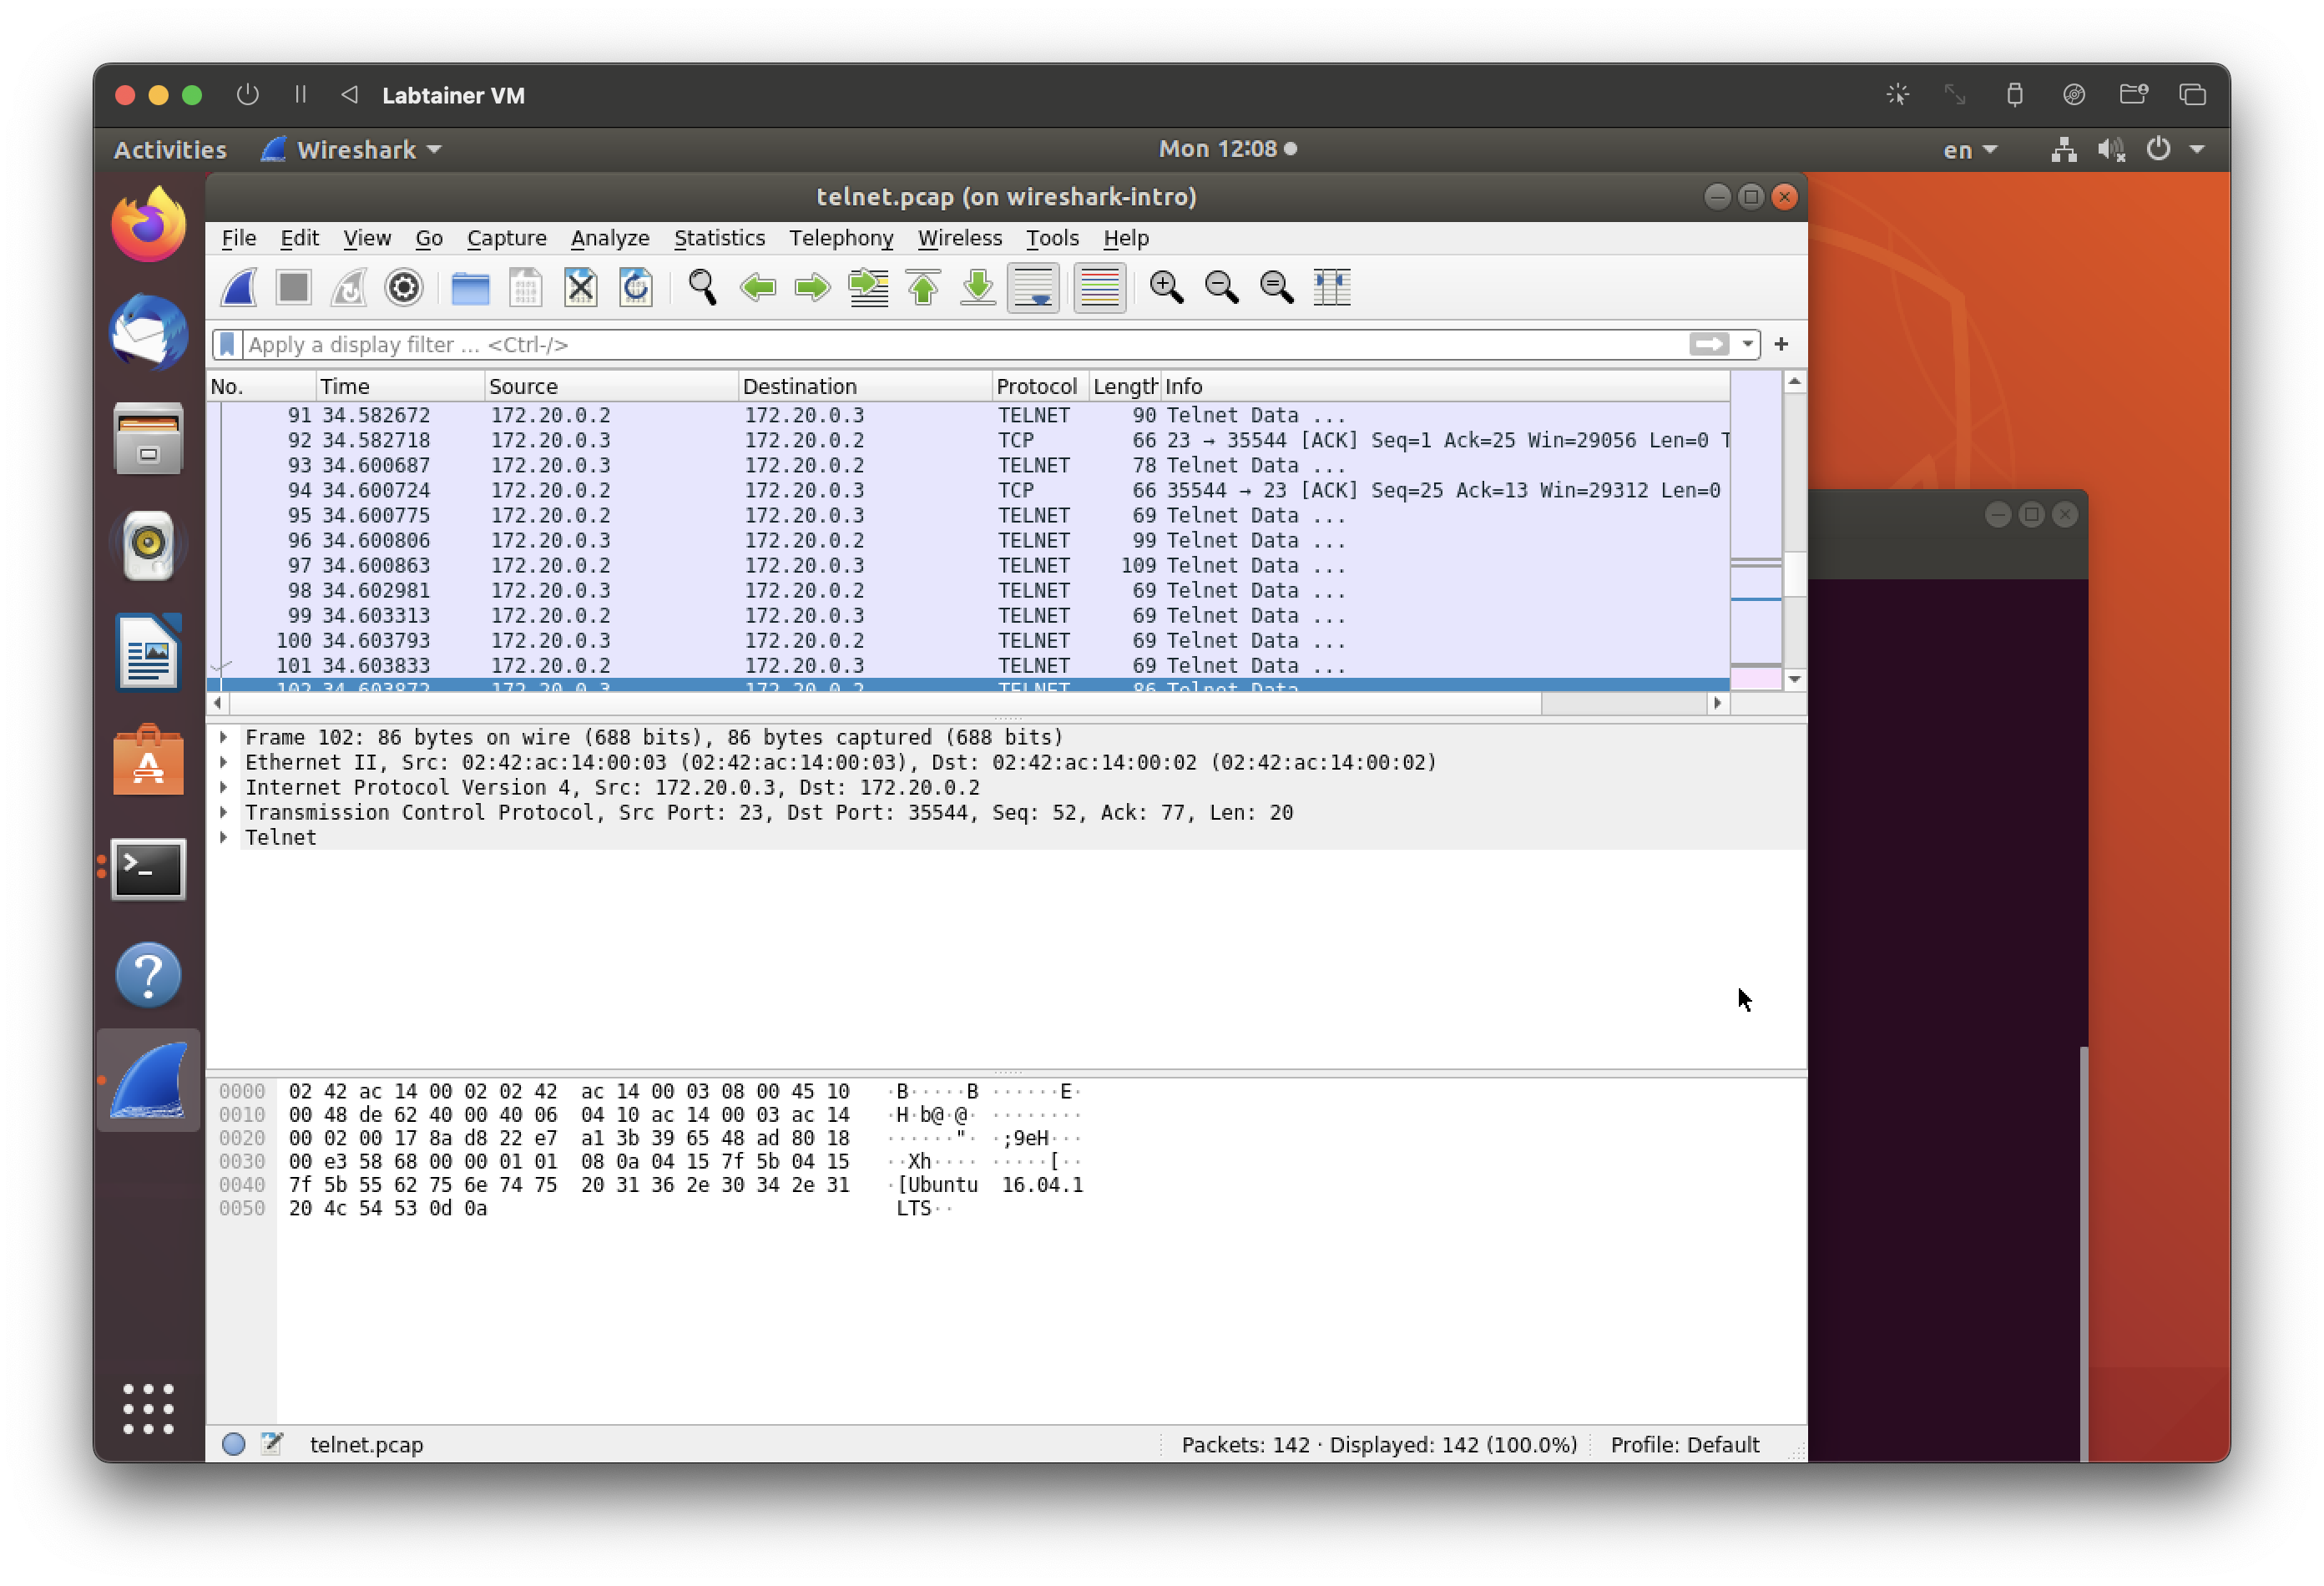
\includegraphics[width=0.8\textwidth]{/Users/marcalstorino/Documents/EMSE/MAJEUR 1 - INFORMATIQUE/Sécurité des Systèmes d'informations/Lab 02/JoaoPedroMarcalStorino_Lab02/image/img01.png} % Substituir pelo caminho correto da imagem
\caption{Wireshark interface after opening the telnet.pcap file}
\end{figure}

\subsection*{Step 3: Analyze Telnet Data}
To focus on the Telnet data, apply the following filter in Wireshark:

\begin{verbatim}
telnet.data
\end{verbatim}

This will filter out the unnecessary packets and display only Telnet-related traffic. Locate the packet containing the login attempt with the username \texttt{john}.

Once found, export the specific packet by navigating to \texttt{File -> Export specified packets}, and save the selected packet as \texttt{invalidpassword.pcap}.

% Espaço para a imagem do filtro Telnet e invalid password
\begin{figure}[h!]
\centering
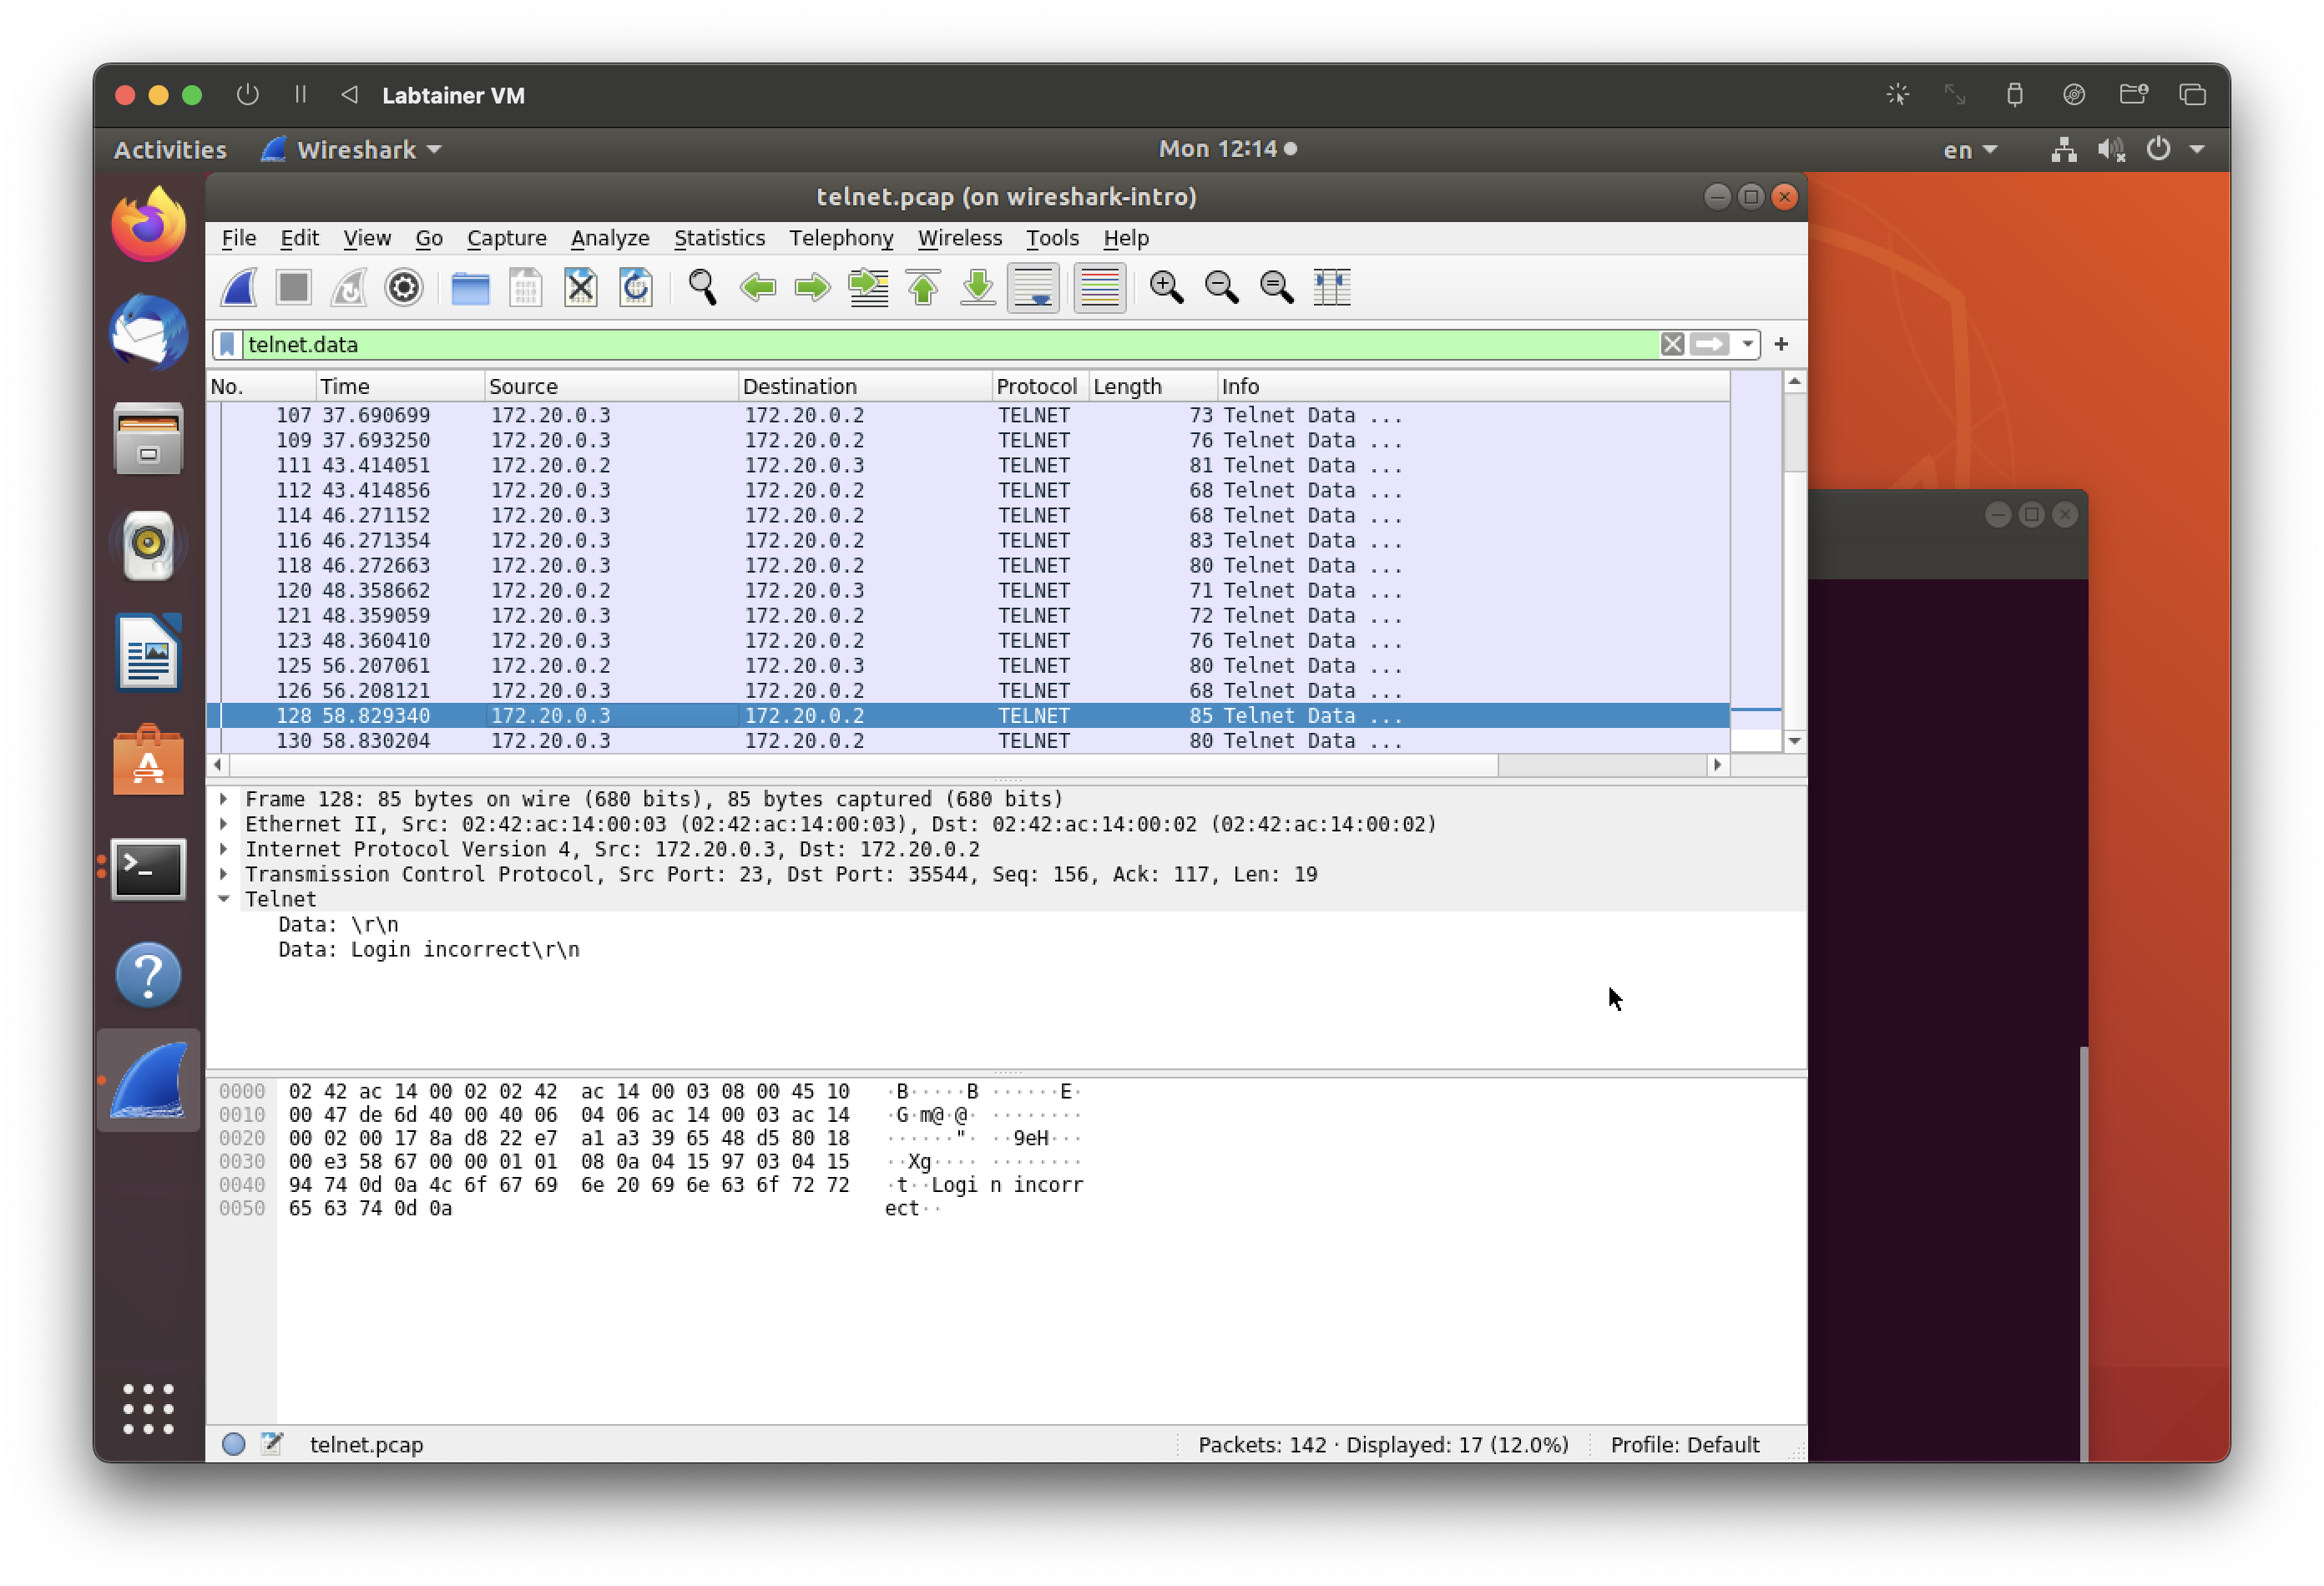
\includegraphics[width=0.8\textwidth]{/Users/marcalstorino/Documents/EMSE/MAJEUR 1 - INFORMATIQUE/Sécurité des Systèmes d'informations/Lab 02/JoaoPedroMarcalStorino_Lab02/image/img02.png} % Substituir pelo caminho correto da imagem
\caption{Filtering Telnet data and exporting invalid password packet}
\end{figure}

\subsection*{Step 4: Explore Further}
After completing the required tasks, I explored additional packets in the Telnet session to gain a better understanding of how the communication was structured. This involved analyzing different types of messages exchanged between the client and the server.

% Espaço para a imagem da parte "explorar mais"
\begin{figure}[h!]
\centering
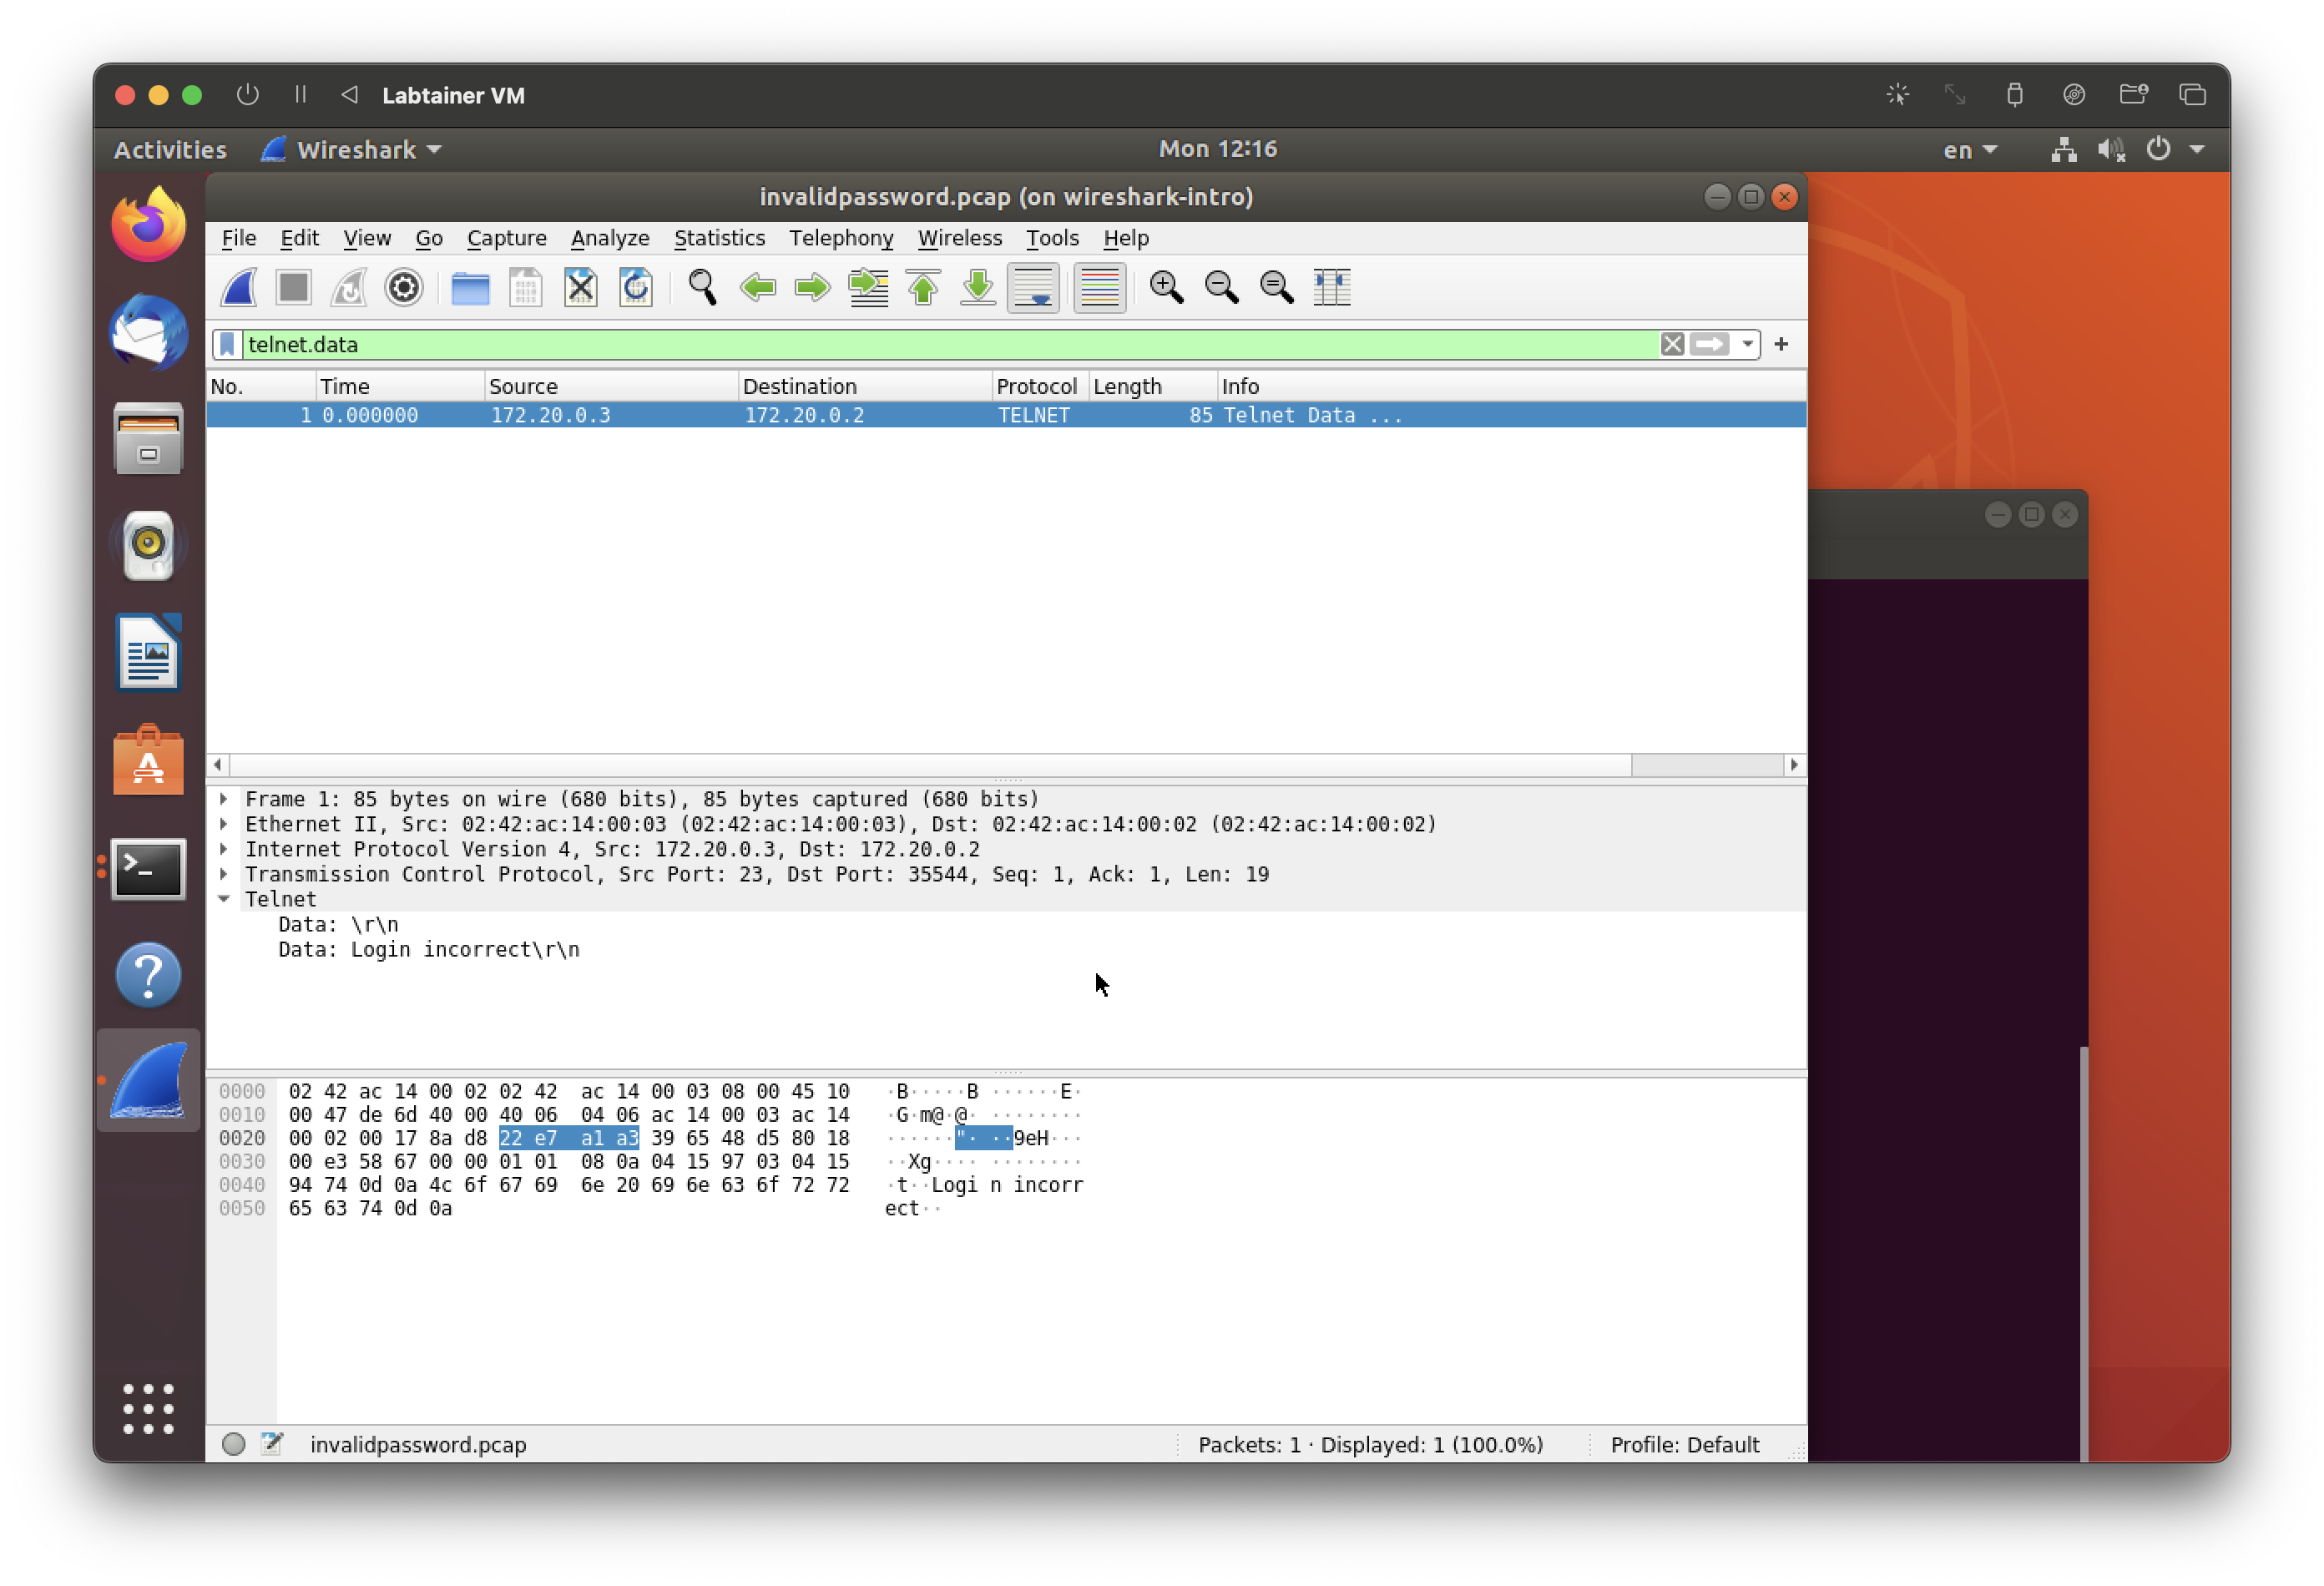
\includegraphics[width=0.7\textwidth]{/Users/marcalstorino/Documents/EMSE/MAJEUR 1 - INFORMATIQUE/Sécurité des Systèmes d'informations/Lab 02/JoaoPedroMarcalStorino_Lab02/image/img03.png} % Substituir pelo caminho correto da imagem
\caption{Exploring additional Telnet packets in Wireshark}
\end{figure}

% Espaço para a última imagem após a análise completa
\begin{figure}[h!]
\centering
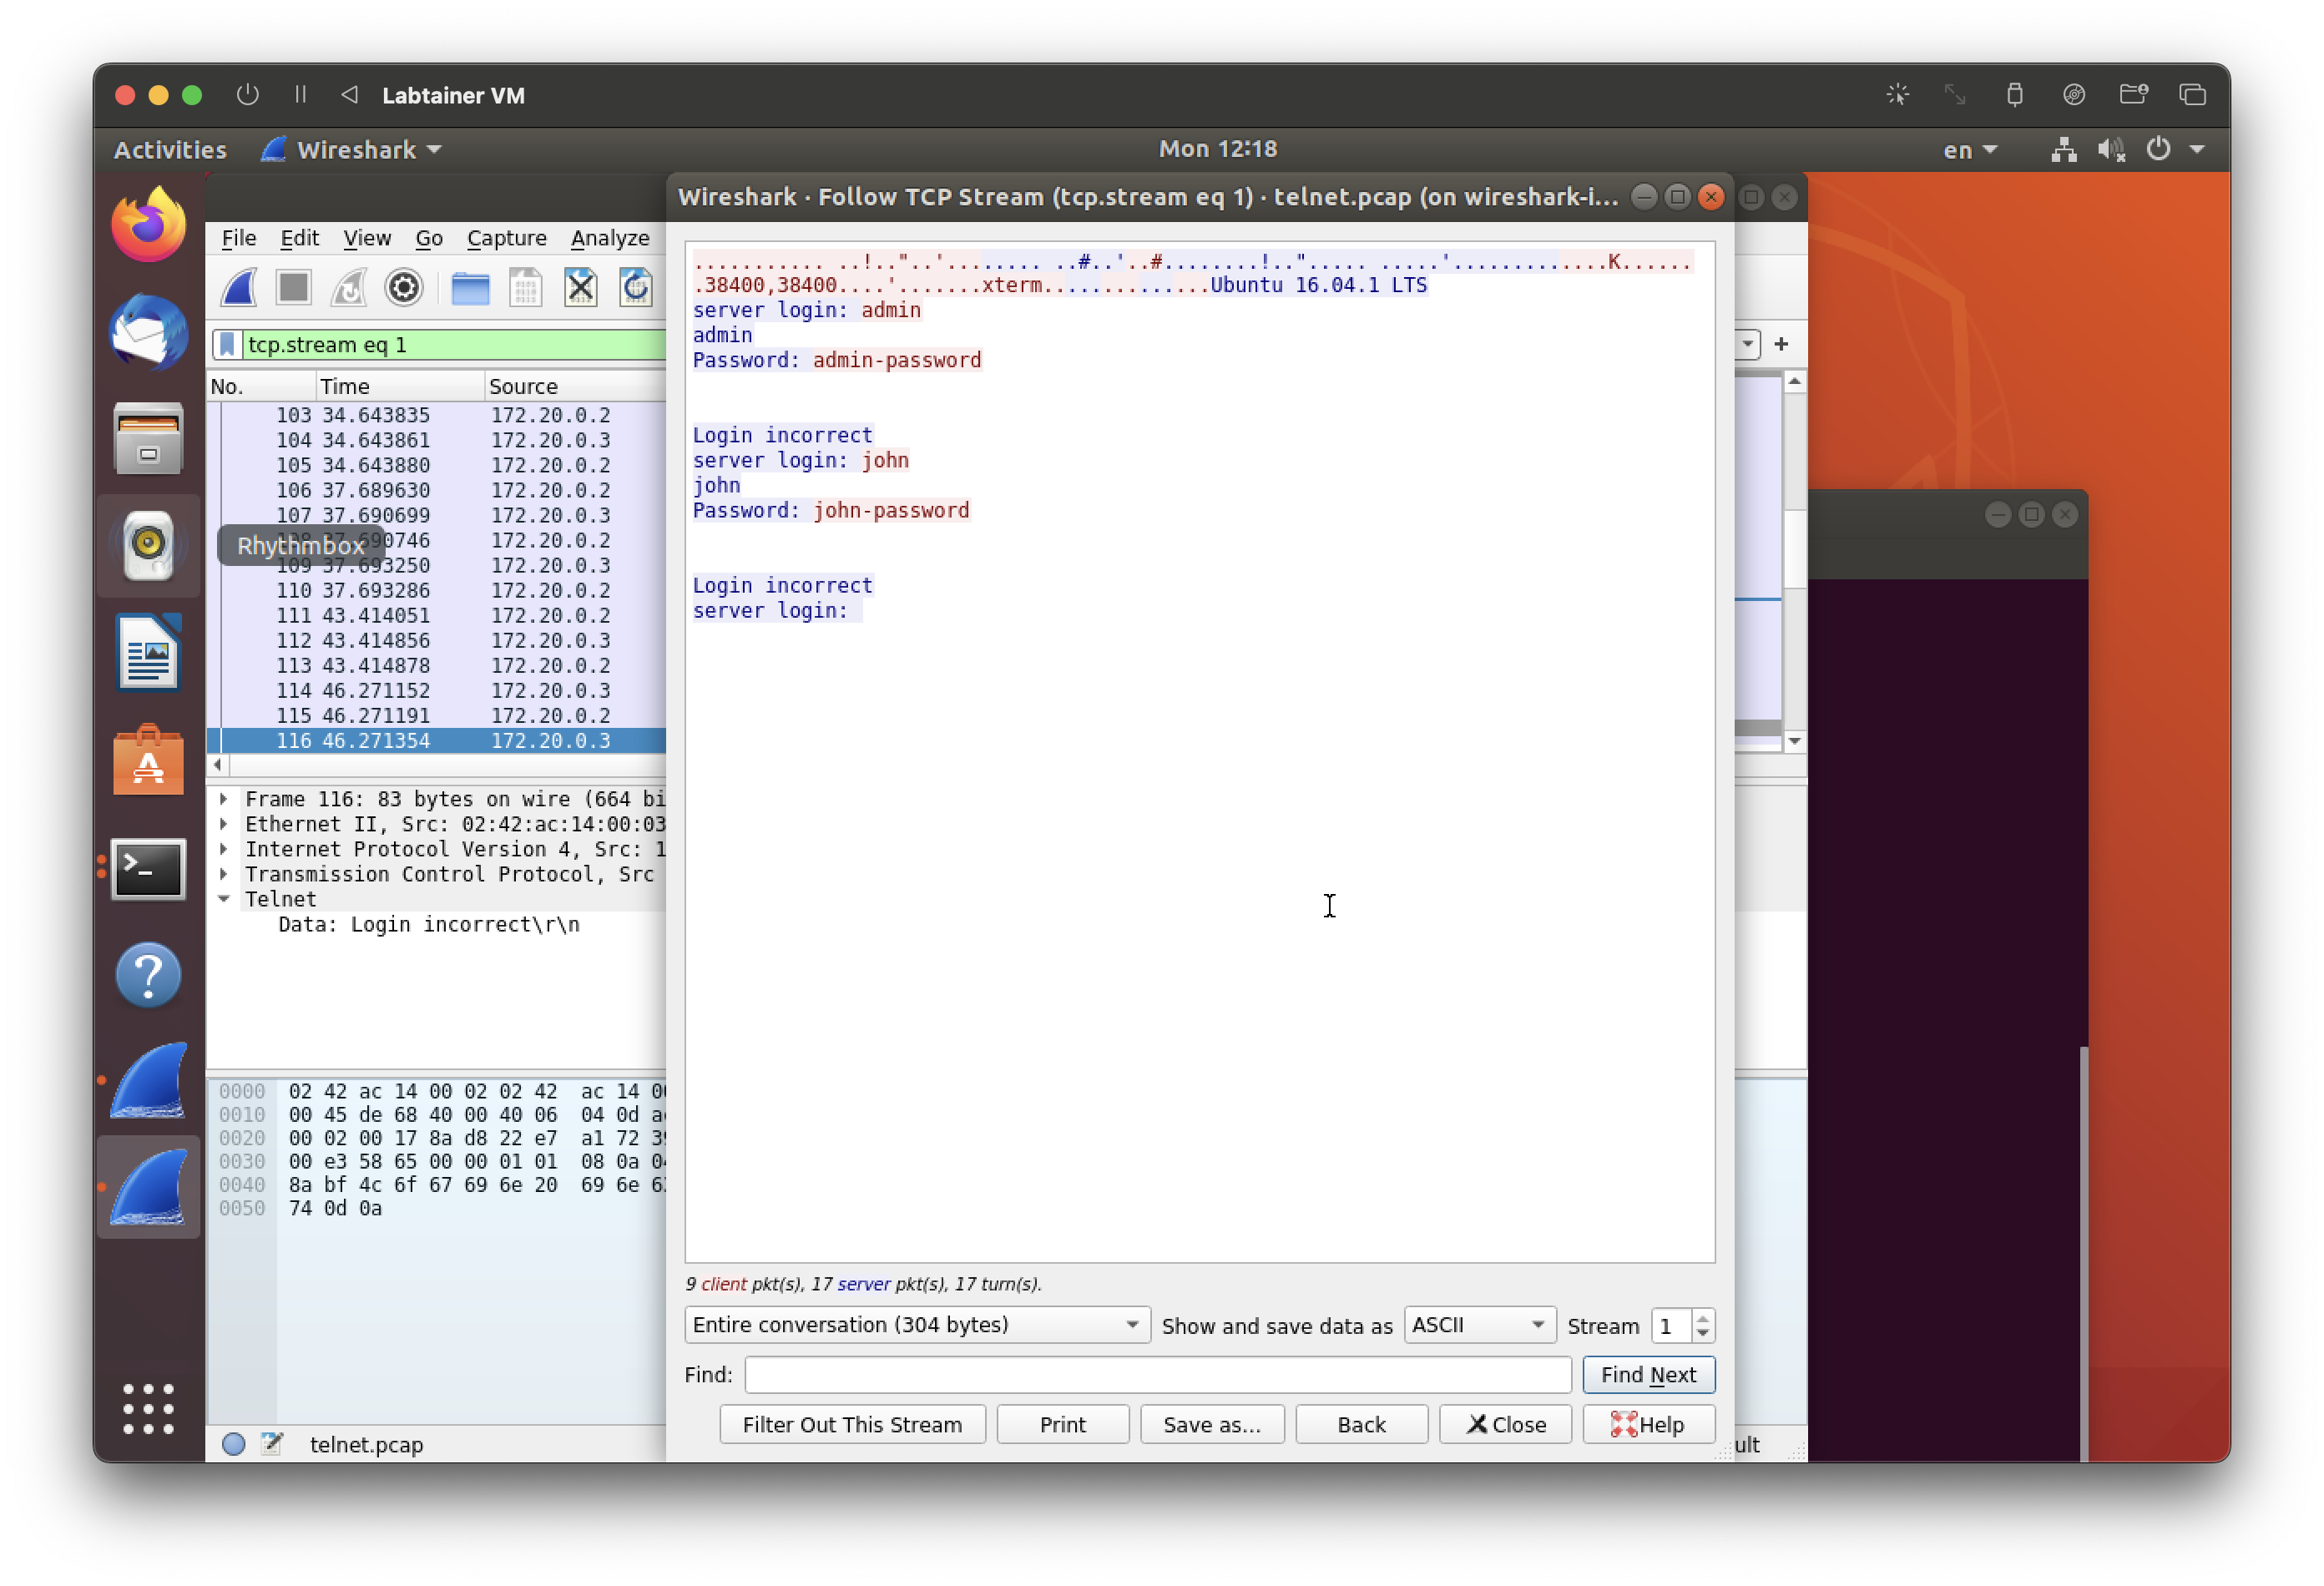
\includegraphics[width=0.7\textwidth]{/Users/marcalstorino/Documents/EMSE/MAJEUR 1 - INFORMATIQUE/Sécurité des Systèmes d'informations/Lab 02/JoaoPedroMarcalStorino_Lab02/image/img04.png} % Substituir pelo caminho correto da imagem
\caption{Full analysis of the Telnet session in Wireshark}
\end{figure}

% Nova seção com a última imagem
\subsection*{Step 5: After analyzing the full Telnet session}
After analyzing the complete Telnet session, I gained deeper insights into the various stages of communication, from connection establishment to command execution. This allowed me to observe the full range of commands and responses exchanged.

\subsection*{Conclusion}
Throughout this lab, several key skills were developed and demonstrated:

\begin{enumerate}
    \item \textbf{Understanding Wireshark}: The ability to capture, stop, and save network packets was demonstrated successfully.
    \item \textbf{Using Filters}: Filters for TCP, HTTP, and specific IPs or ports were applied effectively to narrow down the packet capture results.
    \item \textbf{HTTP Analysis}: HTTP requests and responses were identified and analyzed, providing insight into how web traffic is transmitted.
    \item \textbf{Protocol Understanding}: Packet headers and fields from common protocols like TCP, UDP, and DNS were interpreted, which enhanced the understanding of these protocols' structures.
    \item \textbf{Exporting Data}: Captured data was saved and exported for future analysis, ensuring that key packets could be reviewed and shared for further study.
\end{enumerate}

These skills will be invaluable for diagnosing network issues and gaining a deeper understanding of network communication processes. By mastering these fundamental concepts, a solid foundation has been laid for more advanced network analysis tasks in the future.

\newpage
\section*{IPTables Lab}

\subsection*{Introduction}
The purpose of this lab is to understand how to configure and manage firewall rules using IPTables. IPTables is a powerful tool for controlling incoming and outgoing network traffic in a Linux-based environment. In this lab, we will create and manage rules to allow or block specific network traffic.

\subsection*{Step 1: Launch the Labtainer Environment}
First, open the terminal and run the following command to launch the Labtainer environment for IPTables:

\begin{verbatim}
labtainer iptables2
\end{verbatim}

After starting the environment, you will have access to two terminals: one for the client and another for the firewall.

% Imagem para step 1
\begin{figure}[h!]
\centering
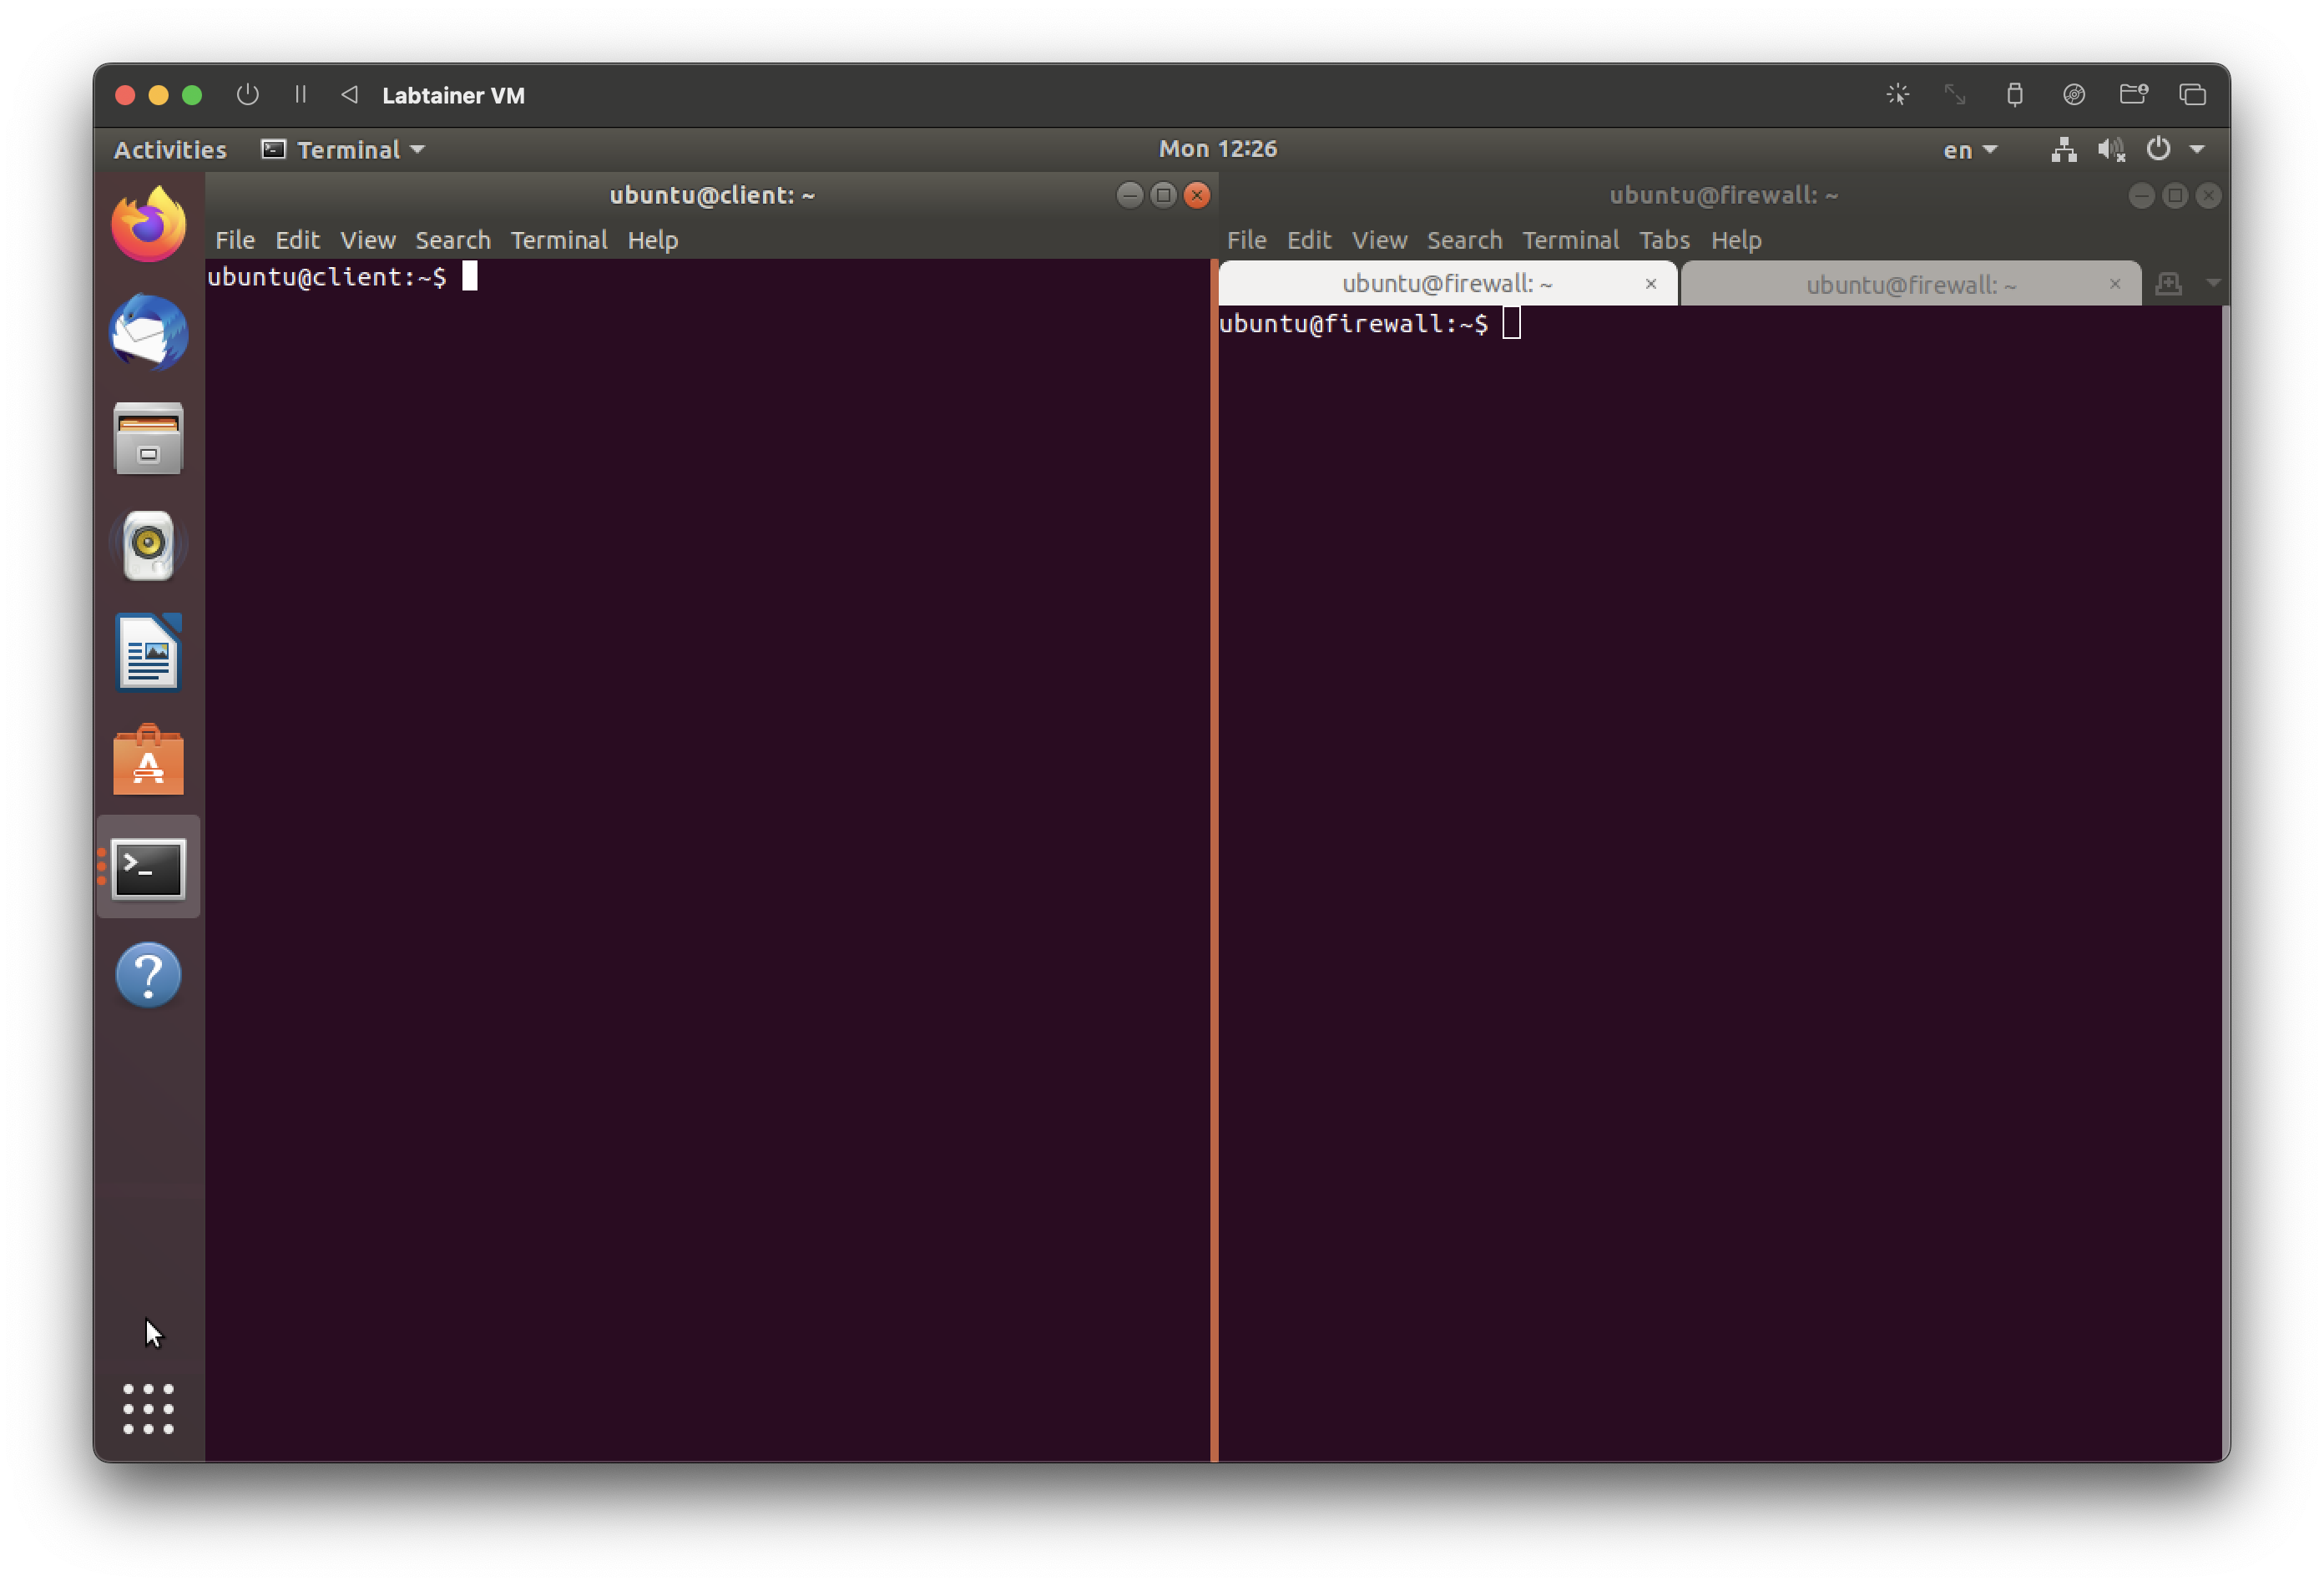
\includegraphics[width=0.8\textwidth]{/Users/marcalstorino/Documents/EMSE/MAJEUR 1 - INFORMATIQUE/Sécurité des Systèmes d'informations/Lab 02/JoaoPedroMarcalStorino_Lab02/image/img05.png} % Substitua pelo caminho correto da imagem
\caption{Launching the Labtainer environment for IPTables}
\end{figure}

\subsection*{Step 2: Analyzing Traffic with Wireshark}
On the firewall terminal, run Wireshark to monitor network traffic:

\begin{verbatim}
wireshark &
\end{verbatim}

Select the \texttt{eth0} interface to begin capturing traffic. From the client terminal, use \texttt{nmap} to scan the server's open ports:

\begin{verbatim}
nmap server
\end{verbatim}

% Imagens para step 2
\begin{figure}[h!]
\centering
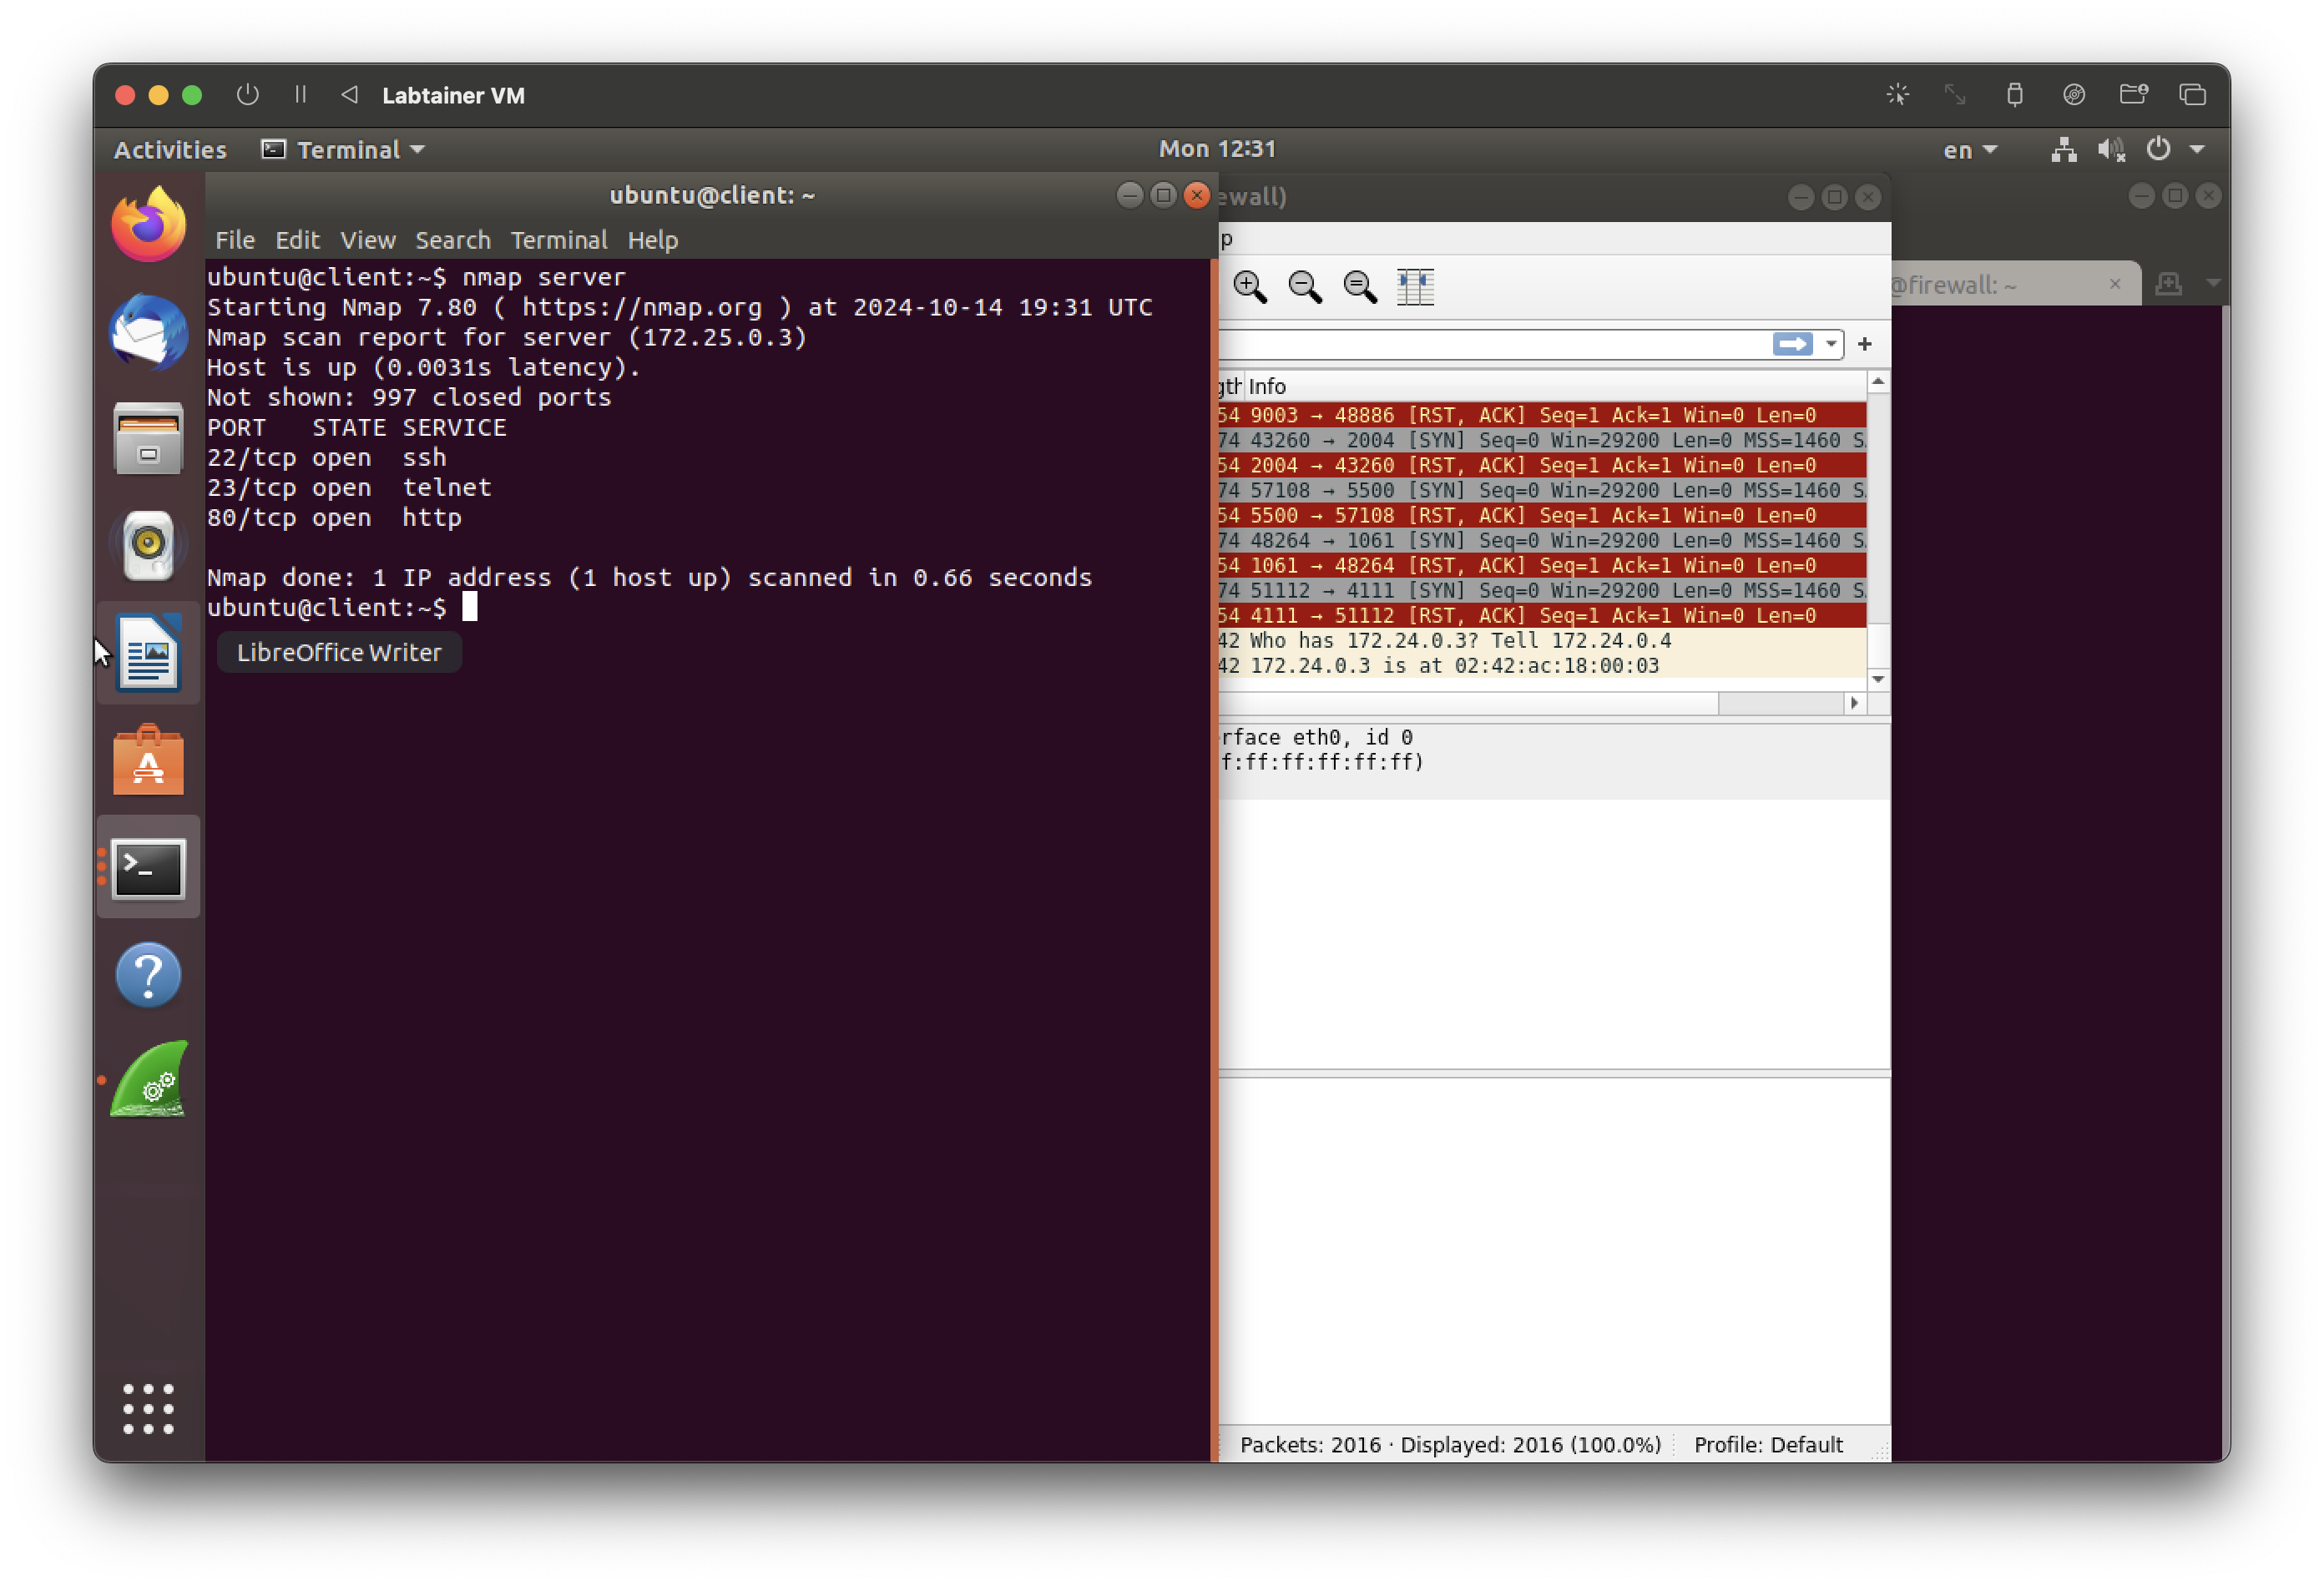
\includegraphics[width=0.8\textwidth]{/Users/marcalstorino/Documents/EMSE/MAJEUR 1 - INFORMATIQUE/Sécurité des Systèmes d'informations/Lab 02/JoaoPedroMarcalStorino_Lab02/image/img06.png} % Substitua pelo caminho correto da imagem
\caption{nmap scanning the server's open ports}
\end{figure}

Next, test HTTP traffic using the following command:

\begin{verbatim}
wget server &
\end{verbatim}

% Imagem para wget
\begin{figure}[h!]
\centering
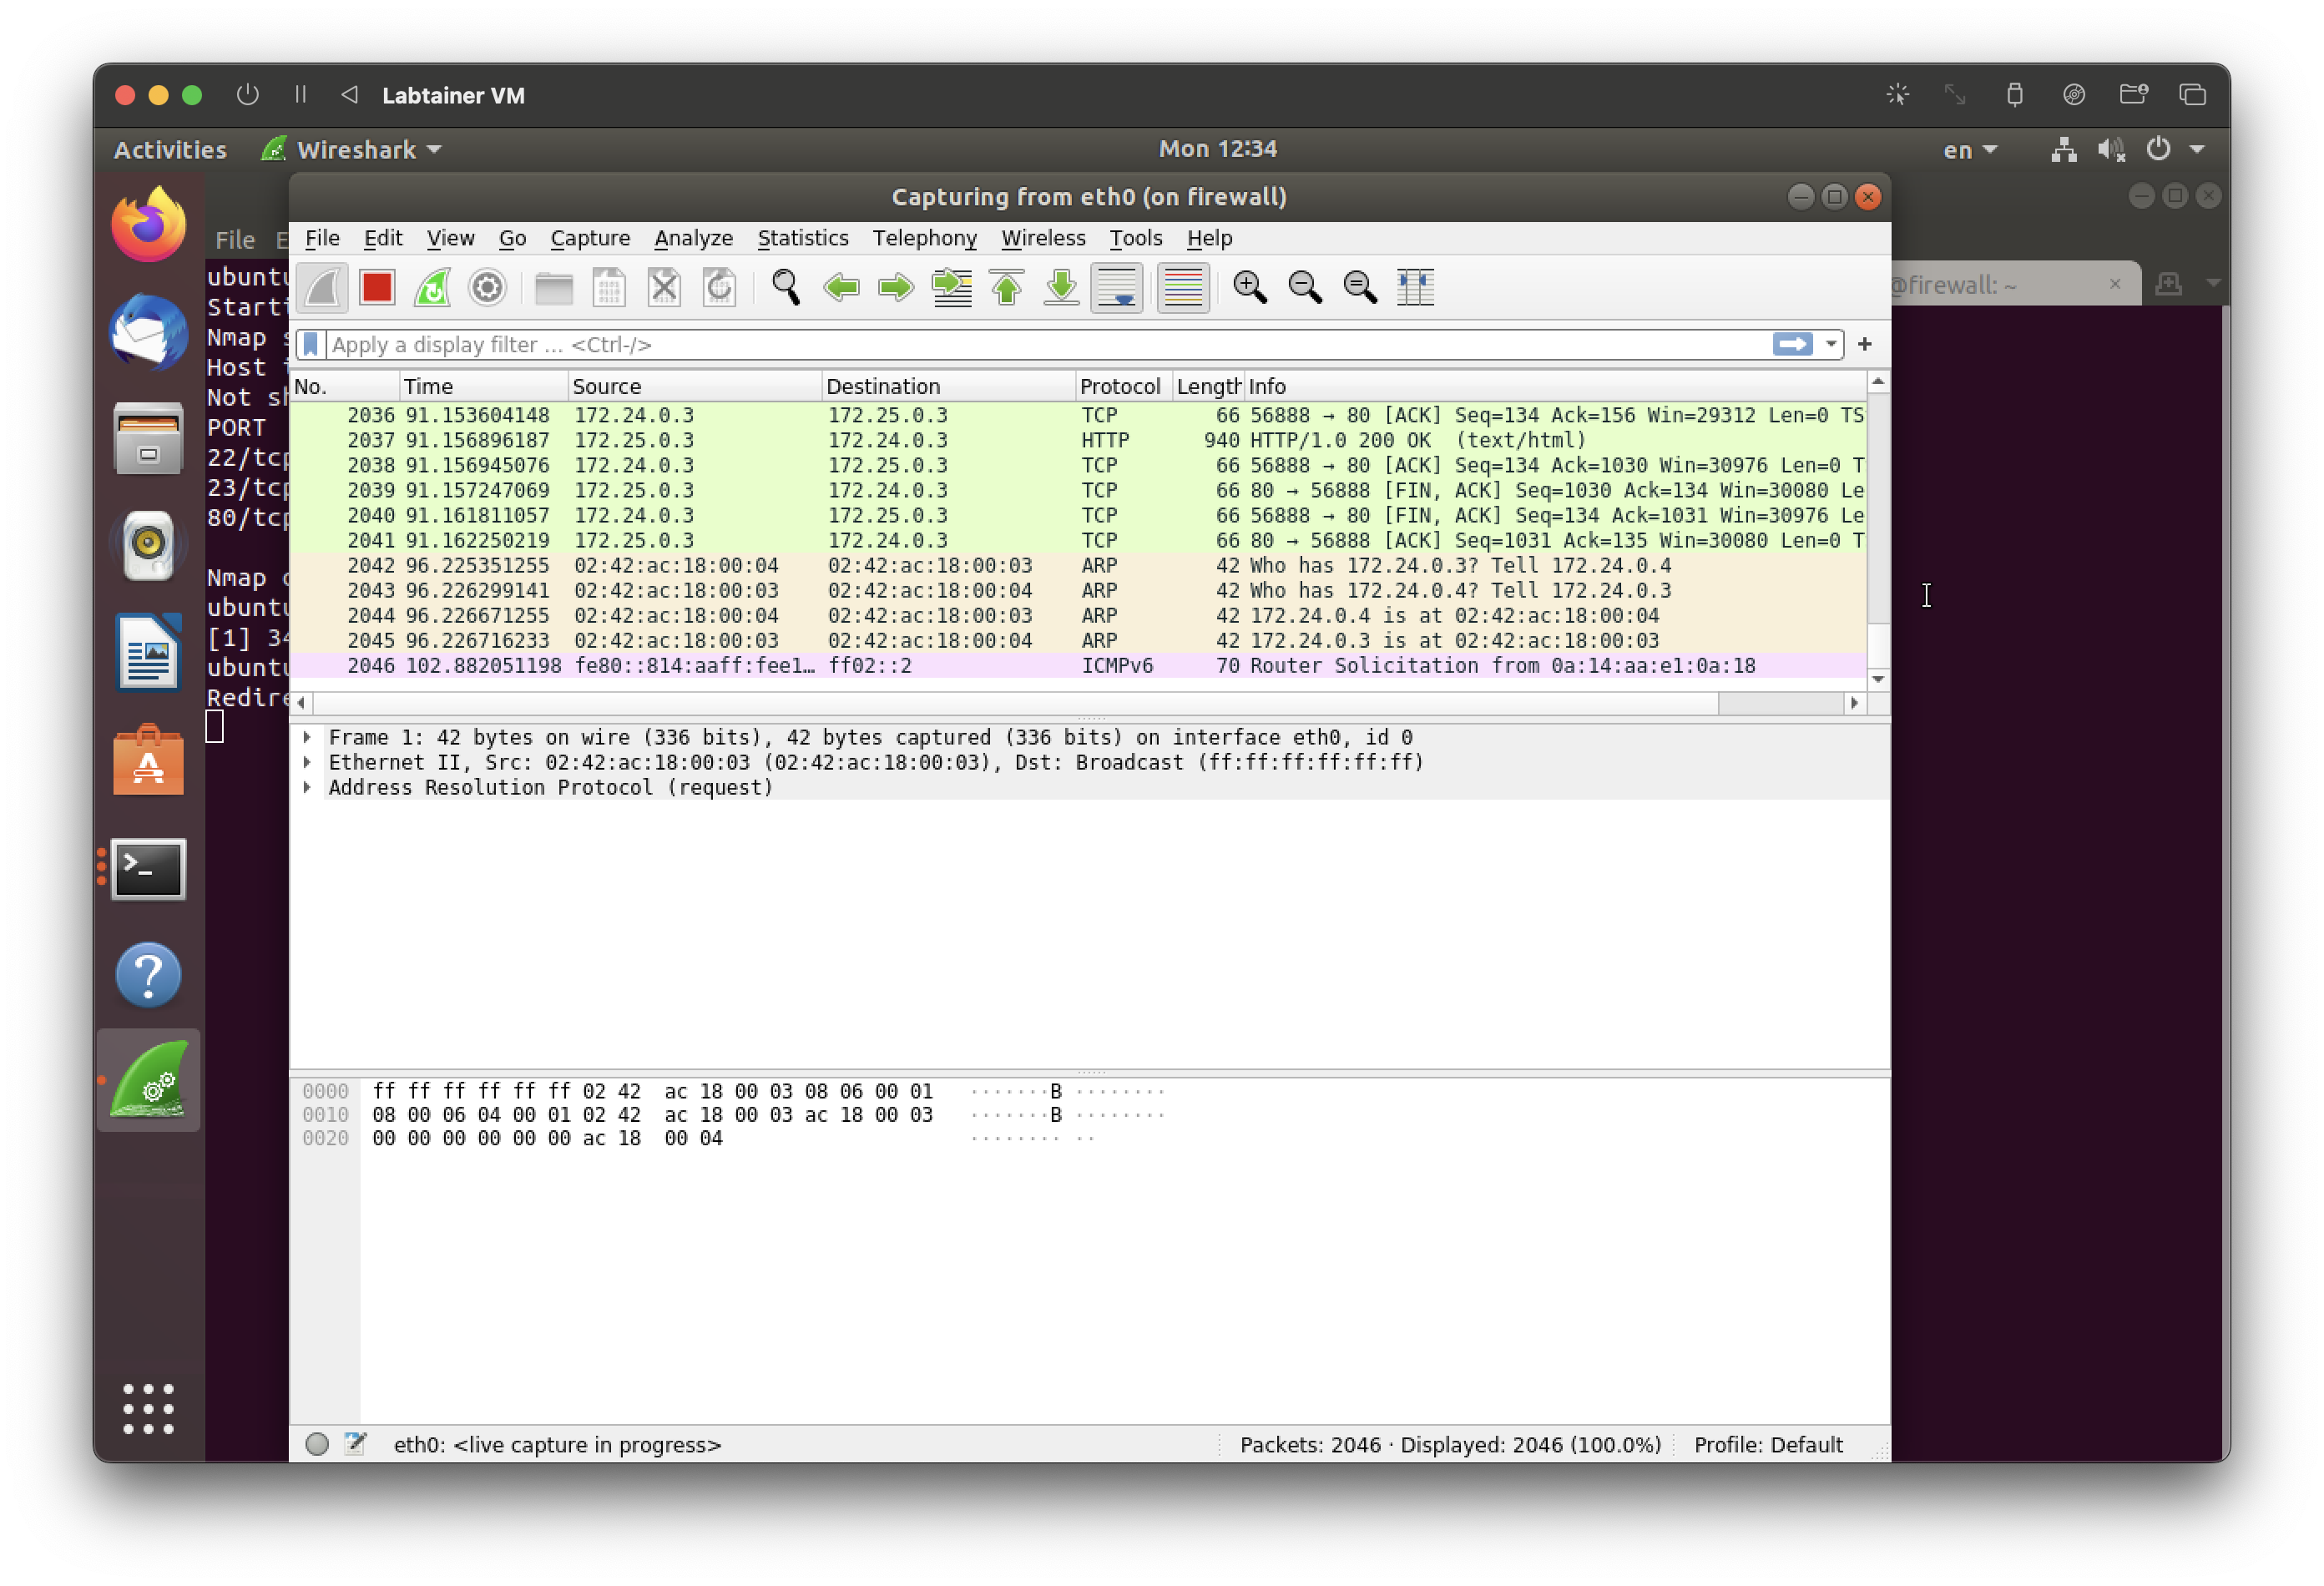
\includegraphics[width=0.8\textwidth]{/Users/marcalstorino/Documents/EMSE/MAJEUR 1 - INFORMATIQUE/Sécurité des Systèmes d'informations/Lab 02/JoaoPedroMarcalStorino_Lab02/image/img07.png} % Substitua pelo caminho correto da imagem
\caption{Testing HTTP traffic using wget}
\end{figure}

Now, test SSH access to the server:

\begin{verbatim}
ssh server
\end{verbatim}

% Imagens para SSH (step 2)
\begin{figure}[h!]
\centering
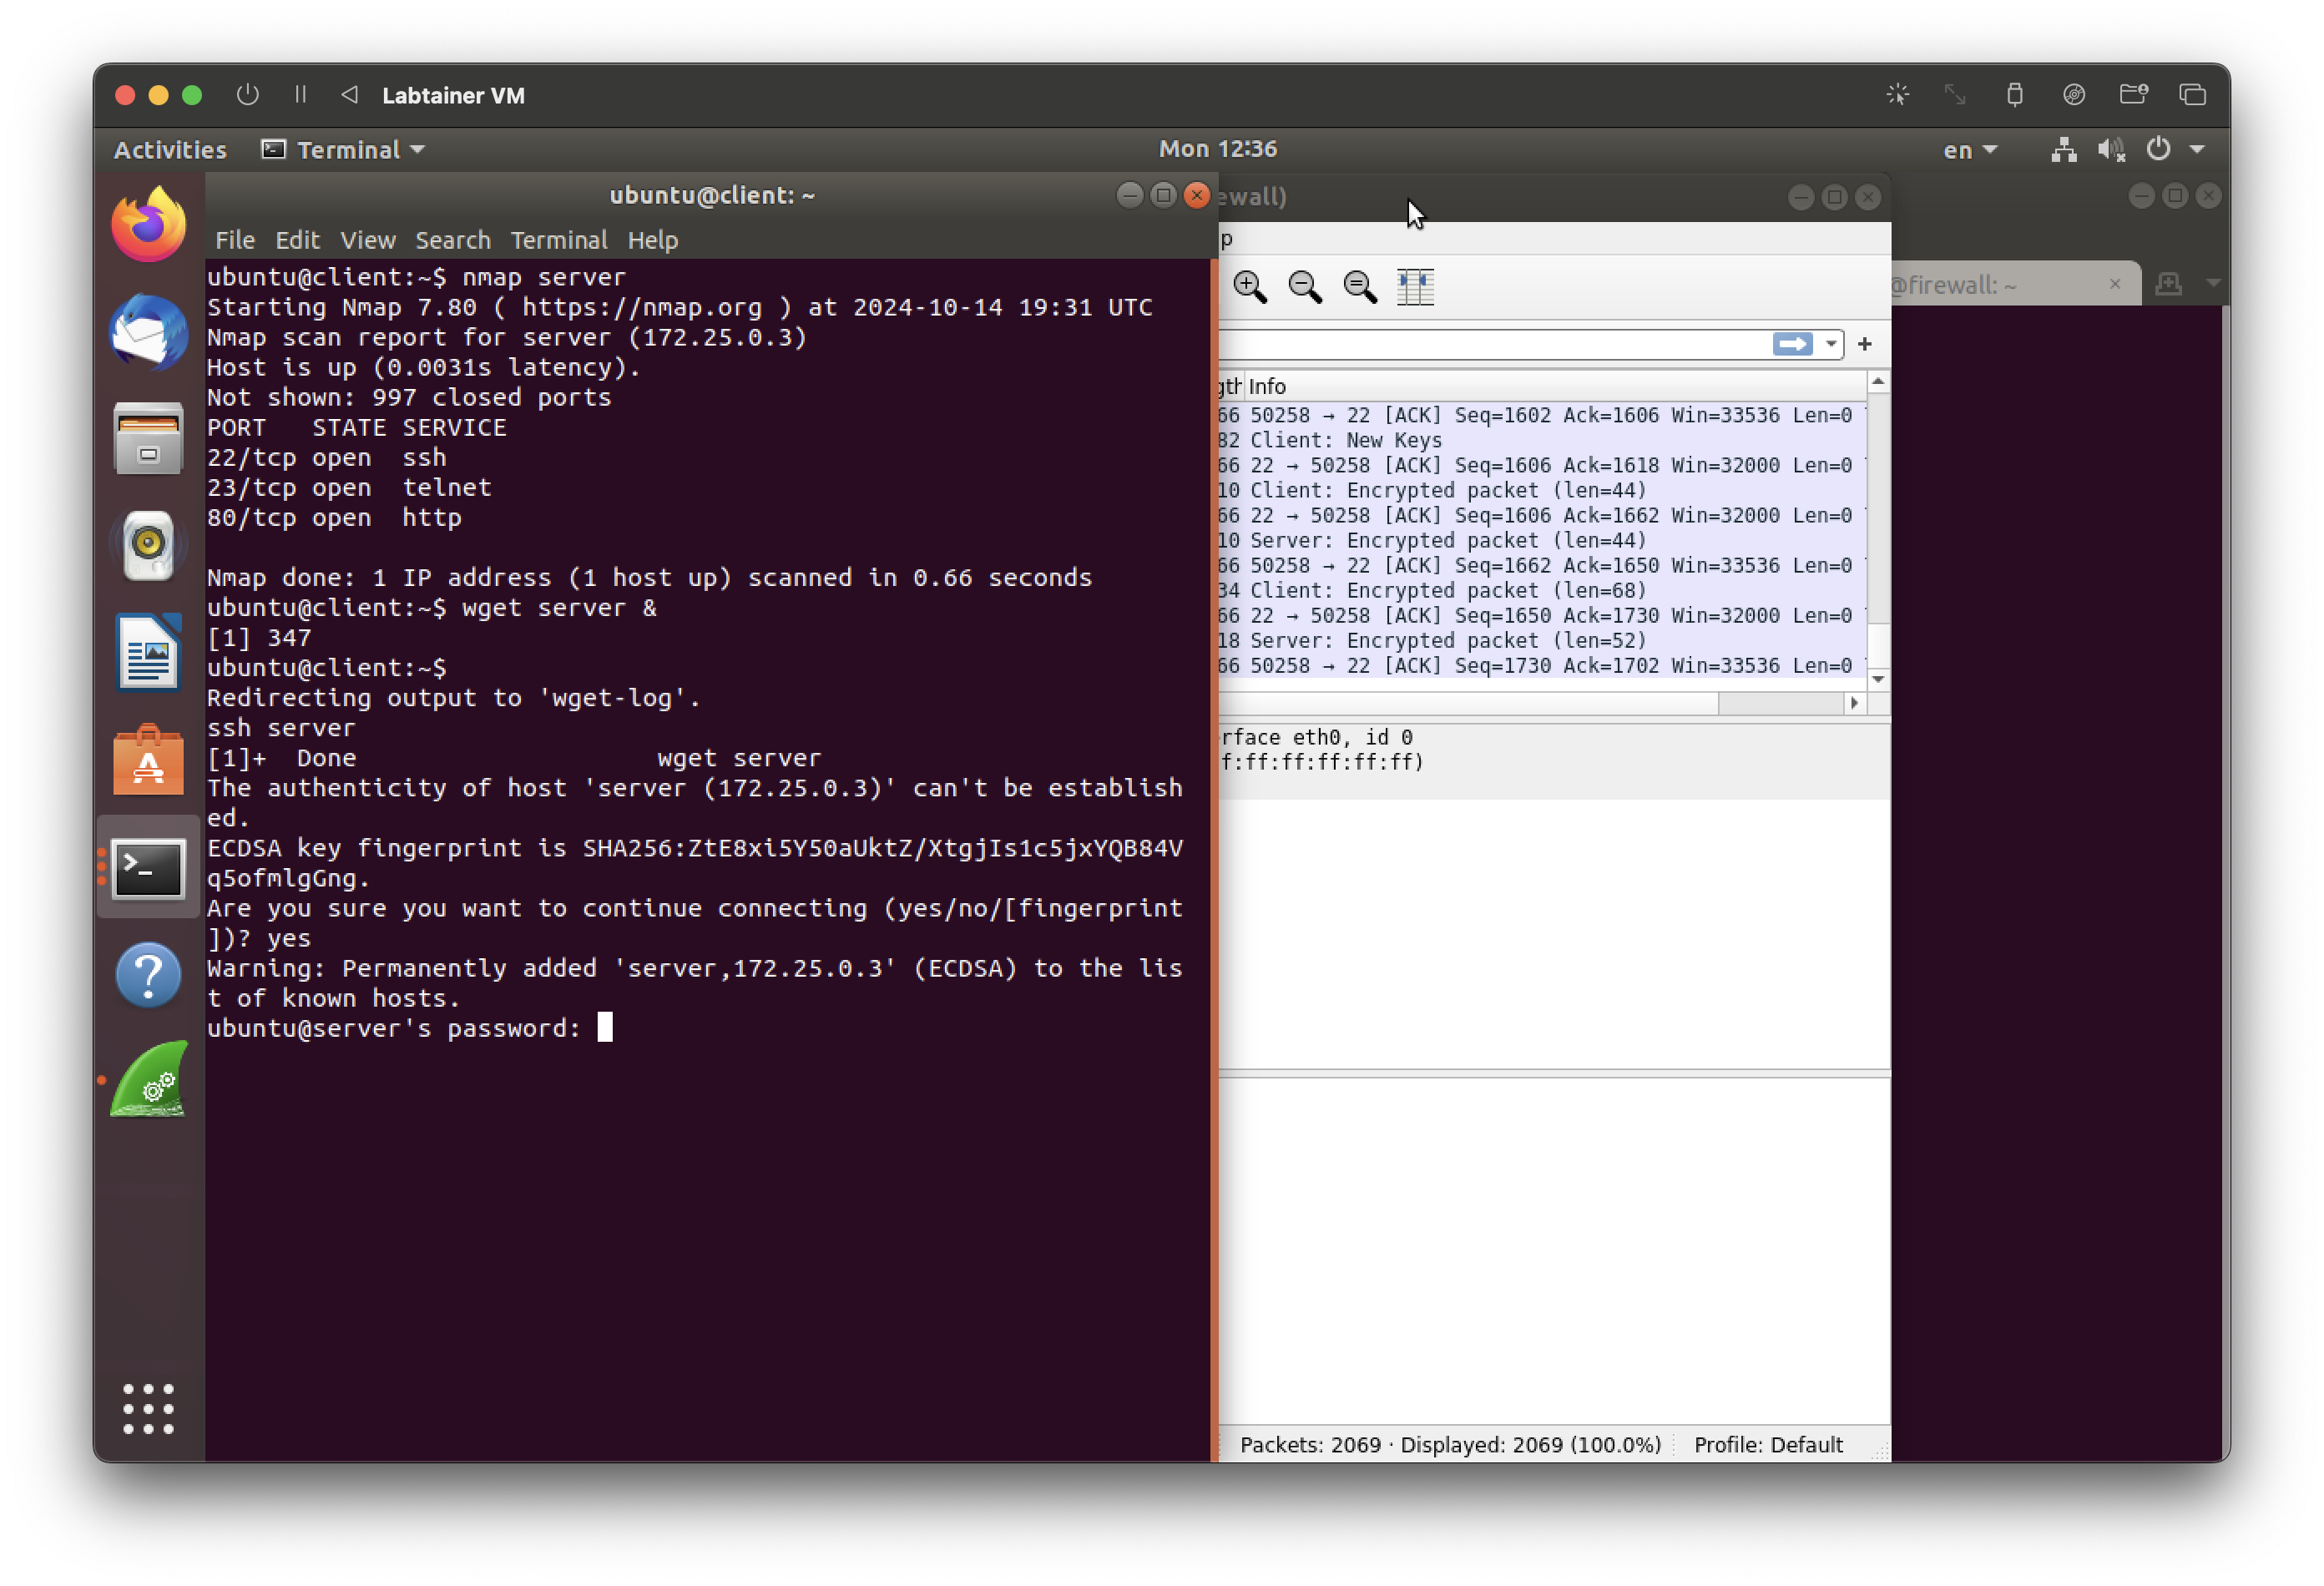
\includegraphics[width=0.8\textwidth]{/Users/marcalstorino/Documents/EMSE/MAJEUR 1 - INFORMATIQUE/Sécurité des Systèmes d'informations/Lab 02/JoaoPedroMarcalStorino_Lab02/image/img08.png} % Substitua pelo caminho correto da imagem
\caption{Testing SSH access to the server}
\end{figure}

% Outra imagem para SSH (step 2)
\begin{figure}[h!]
\centering
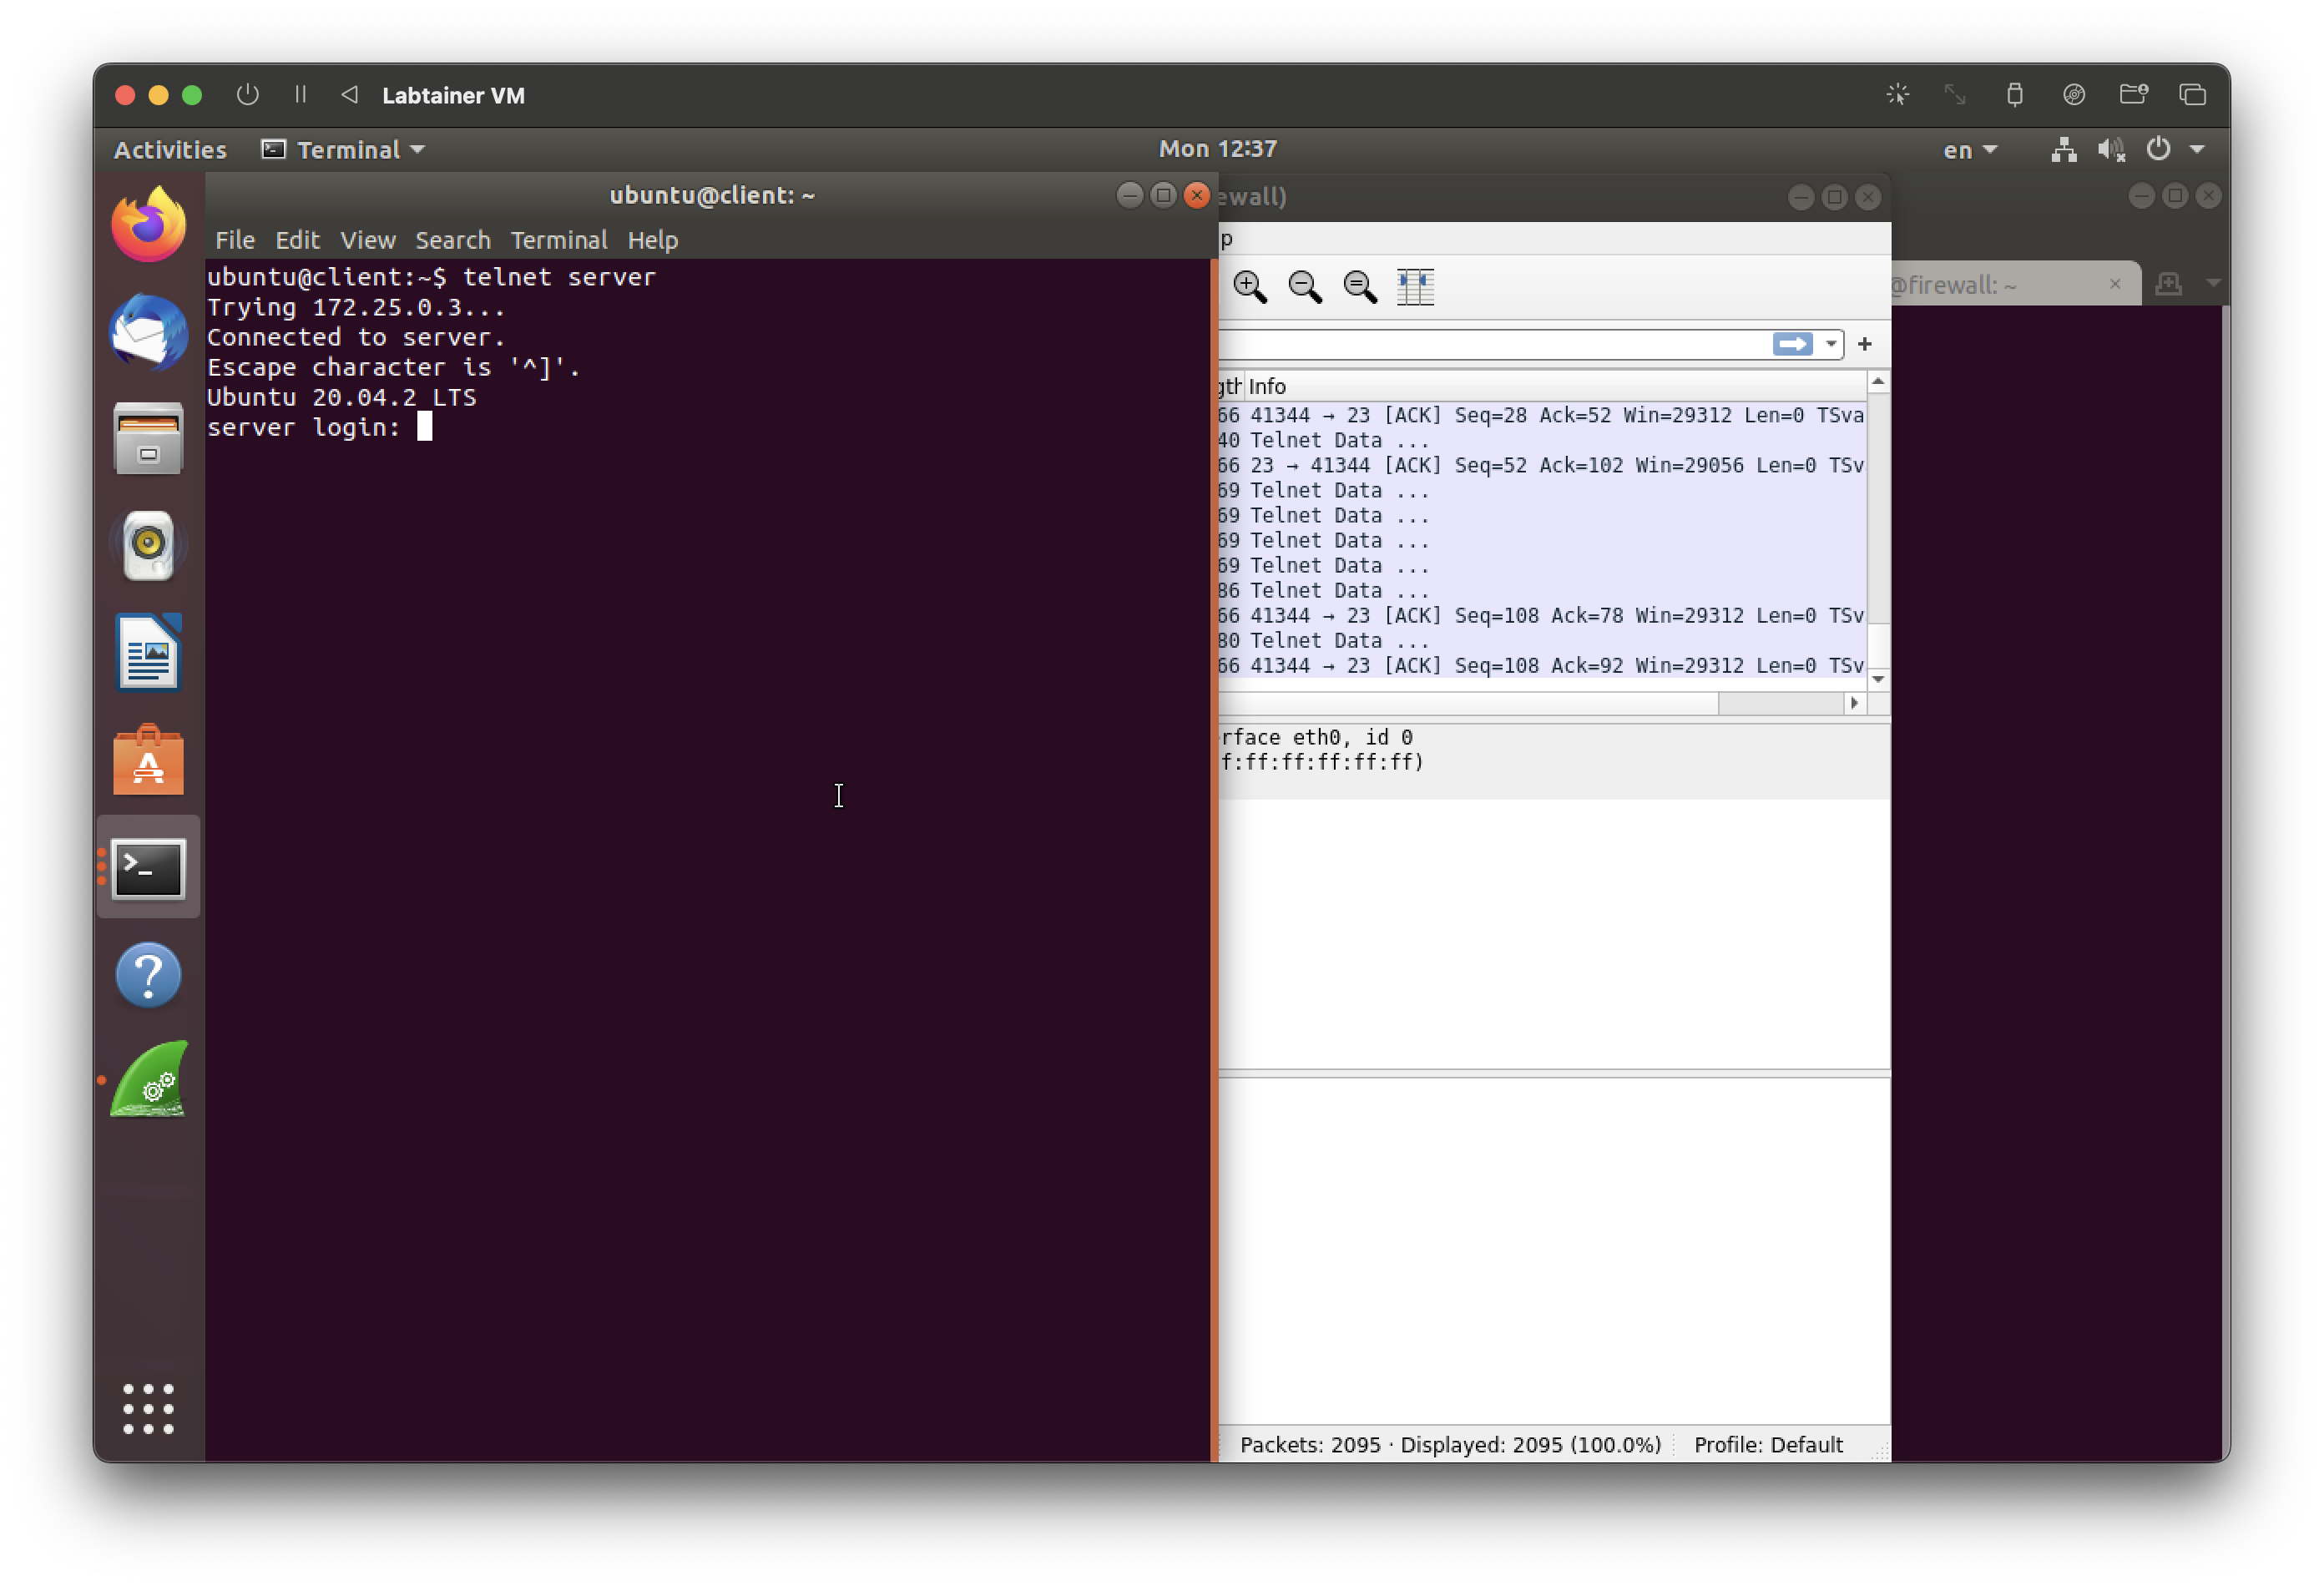
\includegraphics[width=0.8\textwidth]{/Users/marcalstorino/Documents/EMSE/MAJEUR 1 - INFORMATIQUE/Sécurité des Systèmes d'informations/Lab 02/JoaoPedroMarcalStorino_Lab02/image/img09.png} % Substitua pelo caminho correto da imagem
\caption{SSH connection established with the server}
\end{figure}

\subsection*{Step 3: Configure IPTables to Limit Traffic}
Next, configure the firewall to allow only SSH and HTTP traffic, while blocking other types of traffic. On the firewall terminal, execute the following command to apply the IPTables rules:

\begin{verbatim}
sudo ./example_fw.sh
\end{verbatim}

After applying the rules, verify the configuration by running:

\begin{verbatim}
nmap server
\end{verbatim}

% Imagem para step 3 (introduzindo porta 80)
\begin{figure}[h!]
\centering
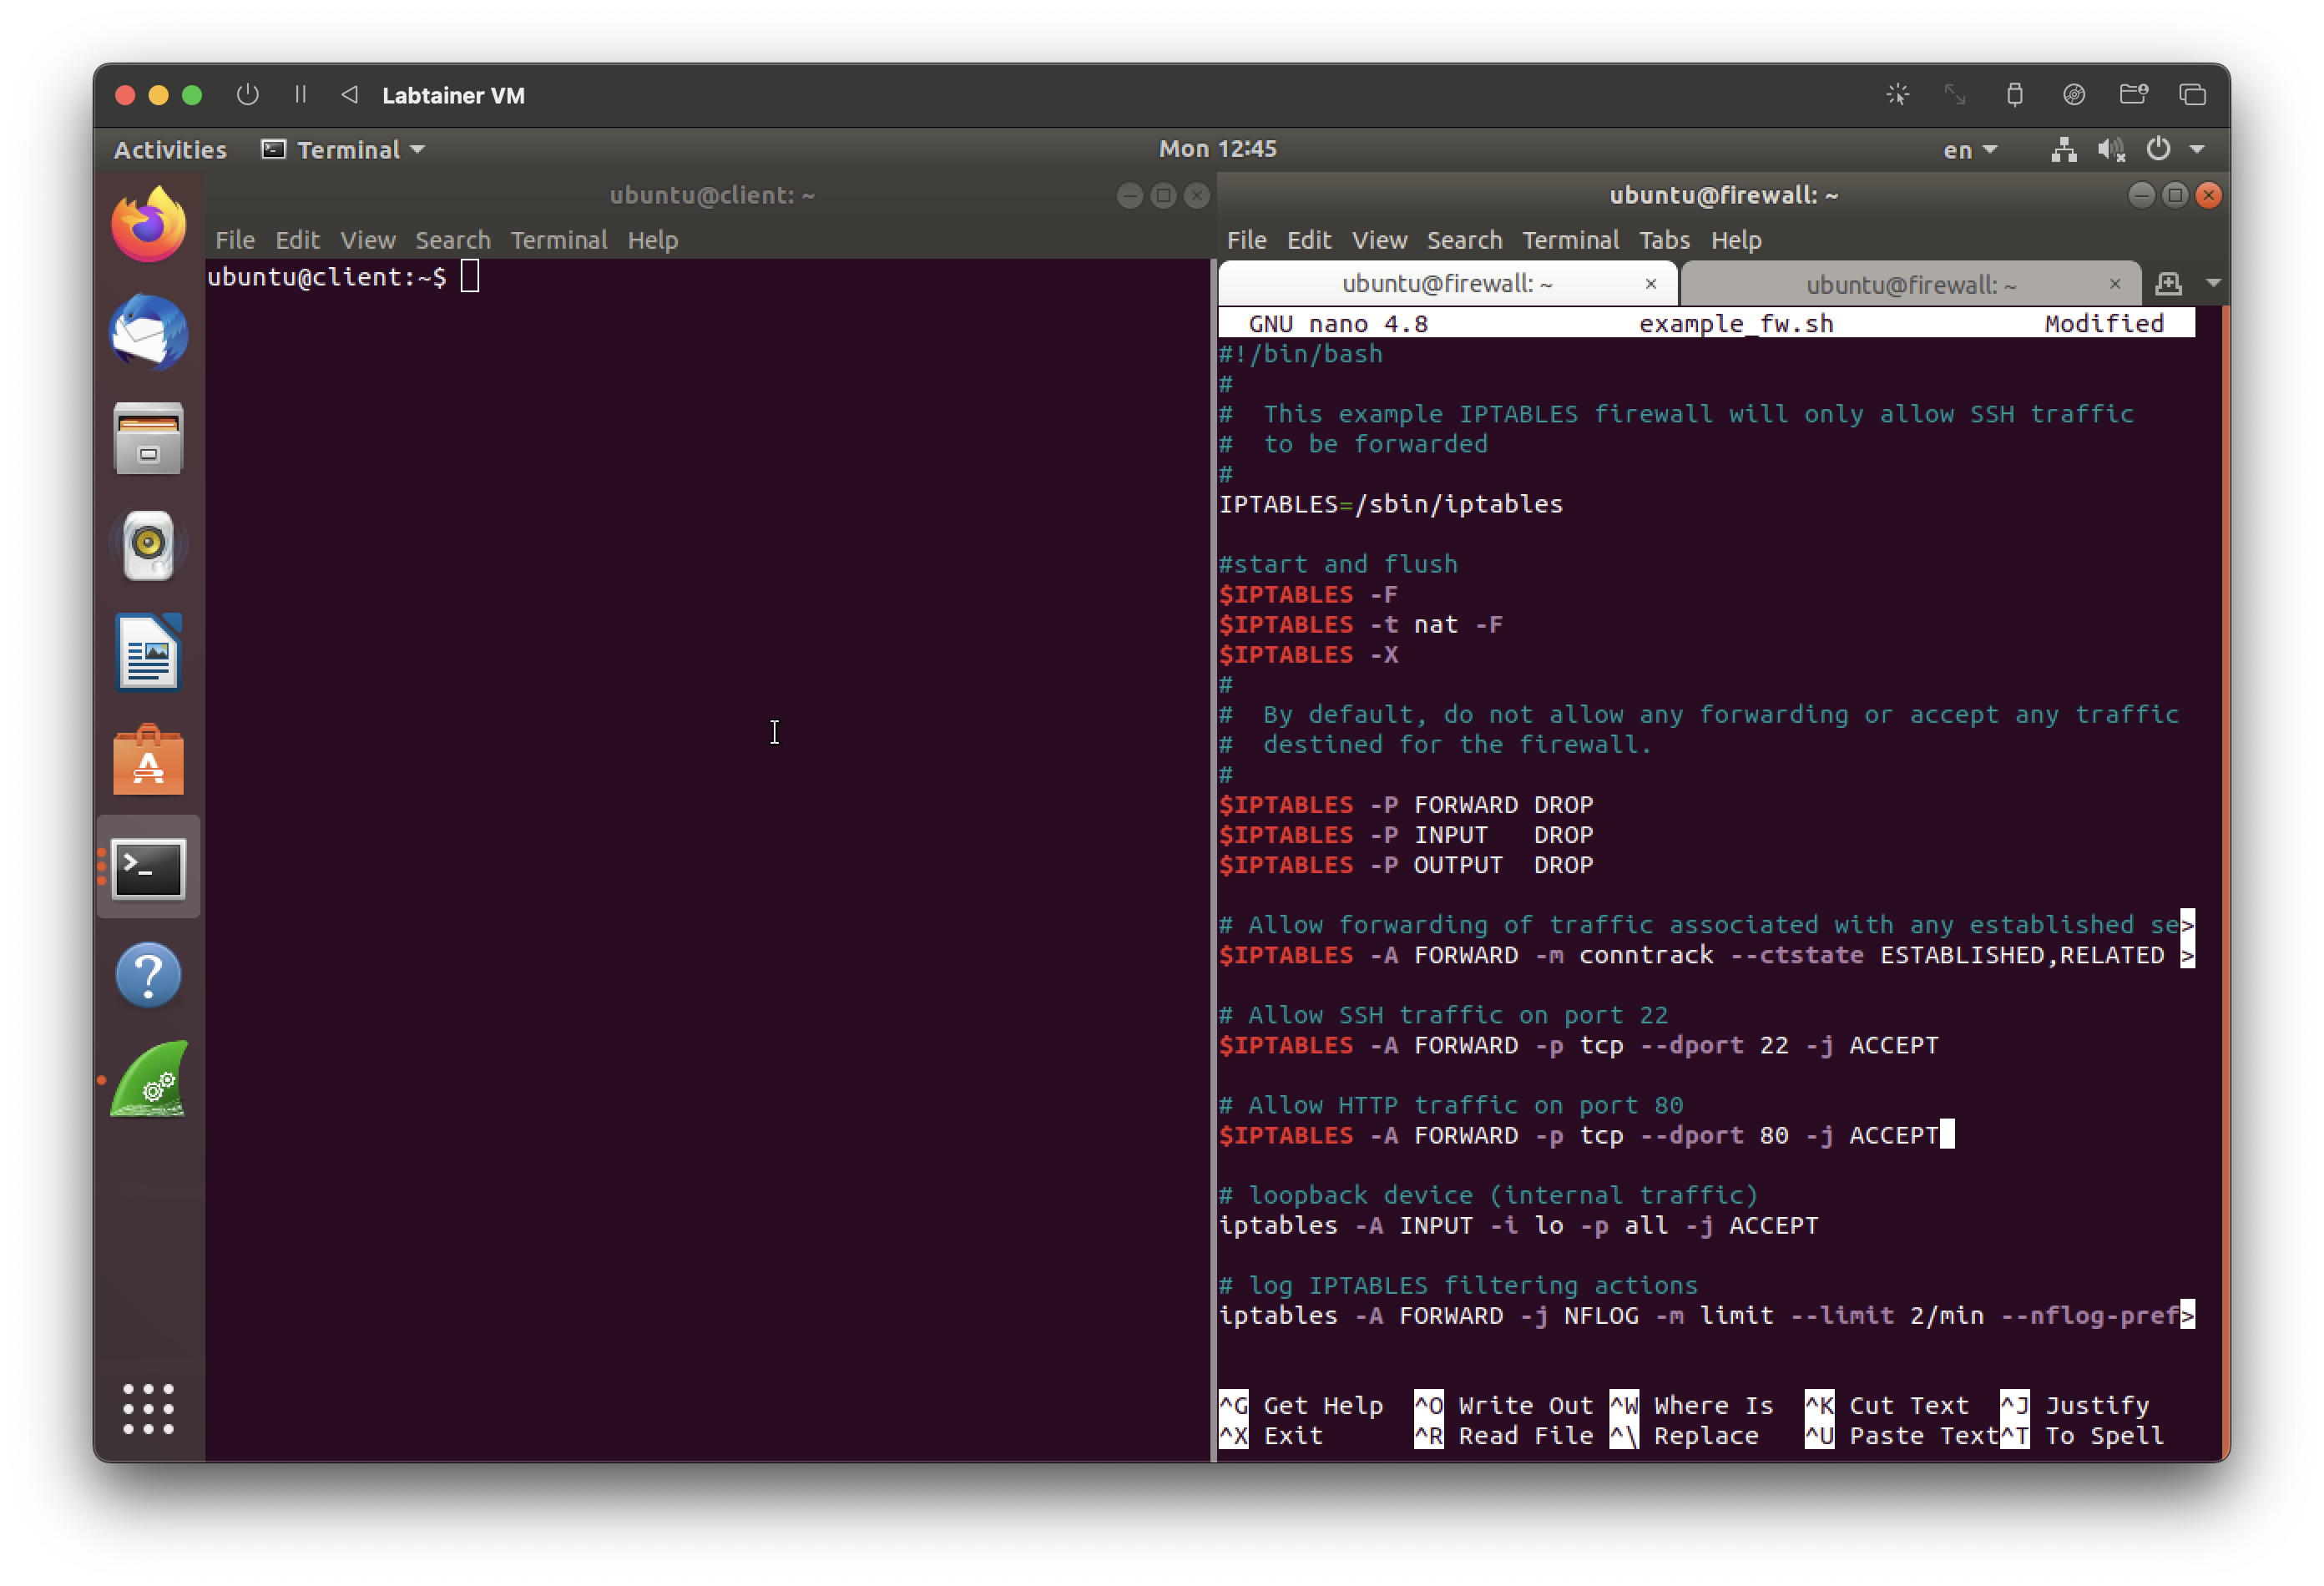
\includegraphics[width=0.8\textwidth]{/Users/marcalstorino/Documents/EMSE/MAJEUR 1 - INFORMATIQUE/Sécurité des Systèmes d'informations/Lab 02/JoaoPedroMarcalStorino_Lab02/image/img10.png} % Substitua pelo caminho correto da imagem
\caption{Configuring IPTables to allow traffic on port 80 (HTTP)}
\end{figure}

% Imagem para step 3 (execução nmap)
\begin{figure}[h!]
\centering
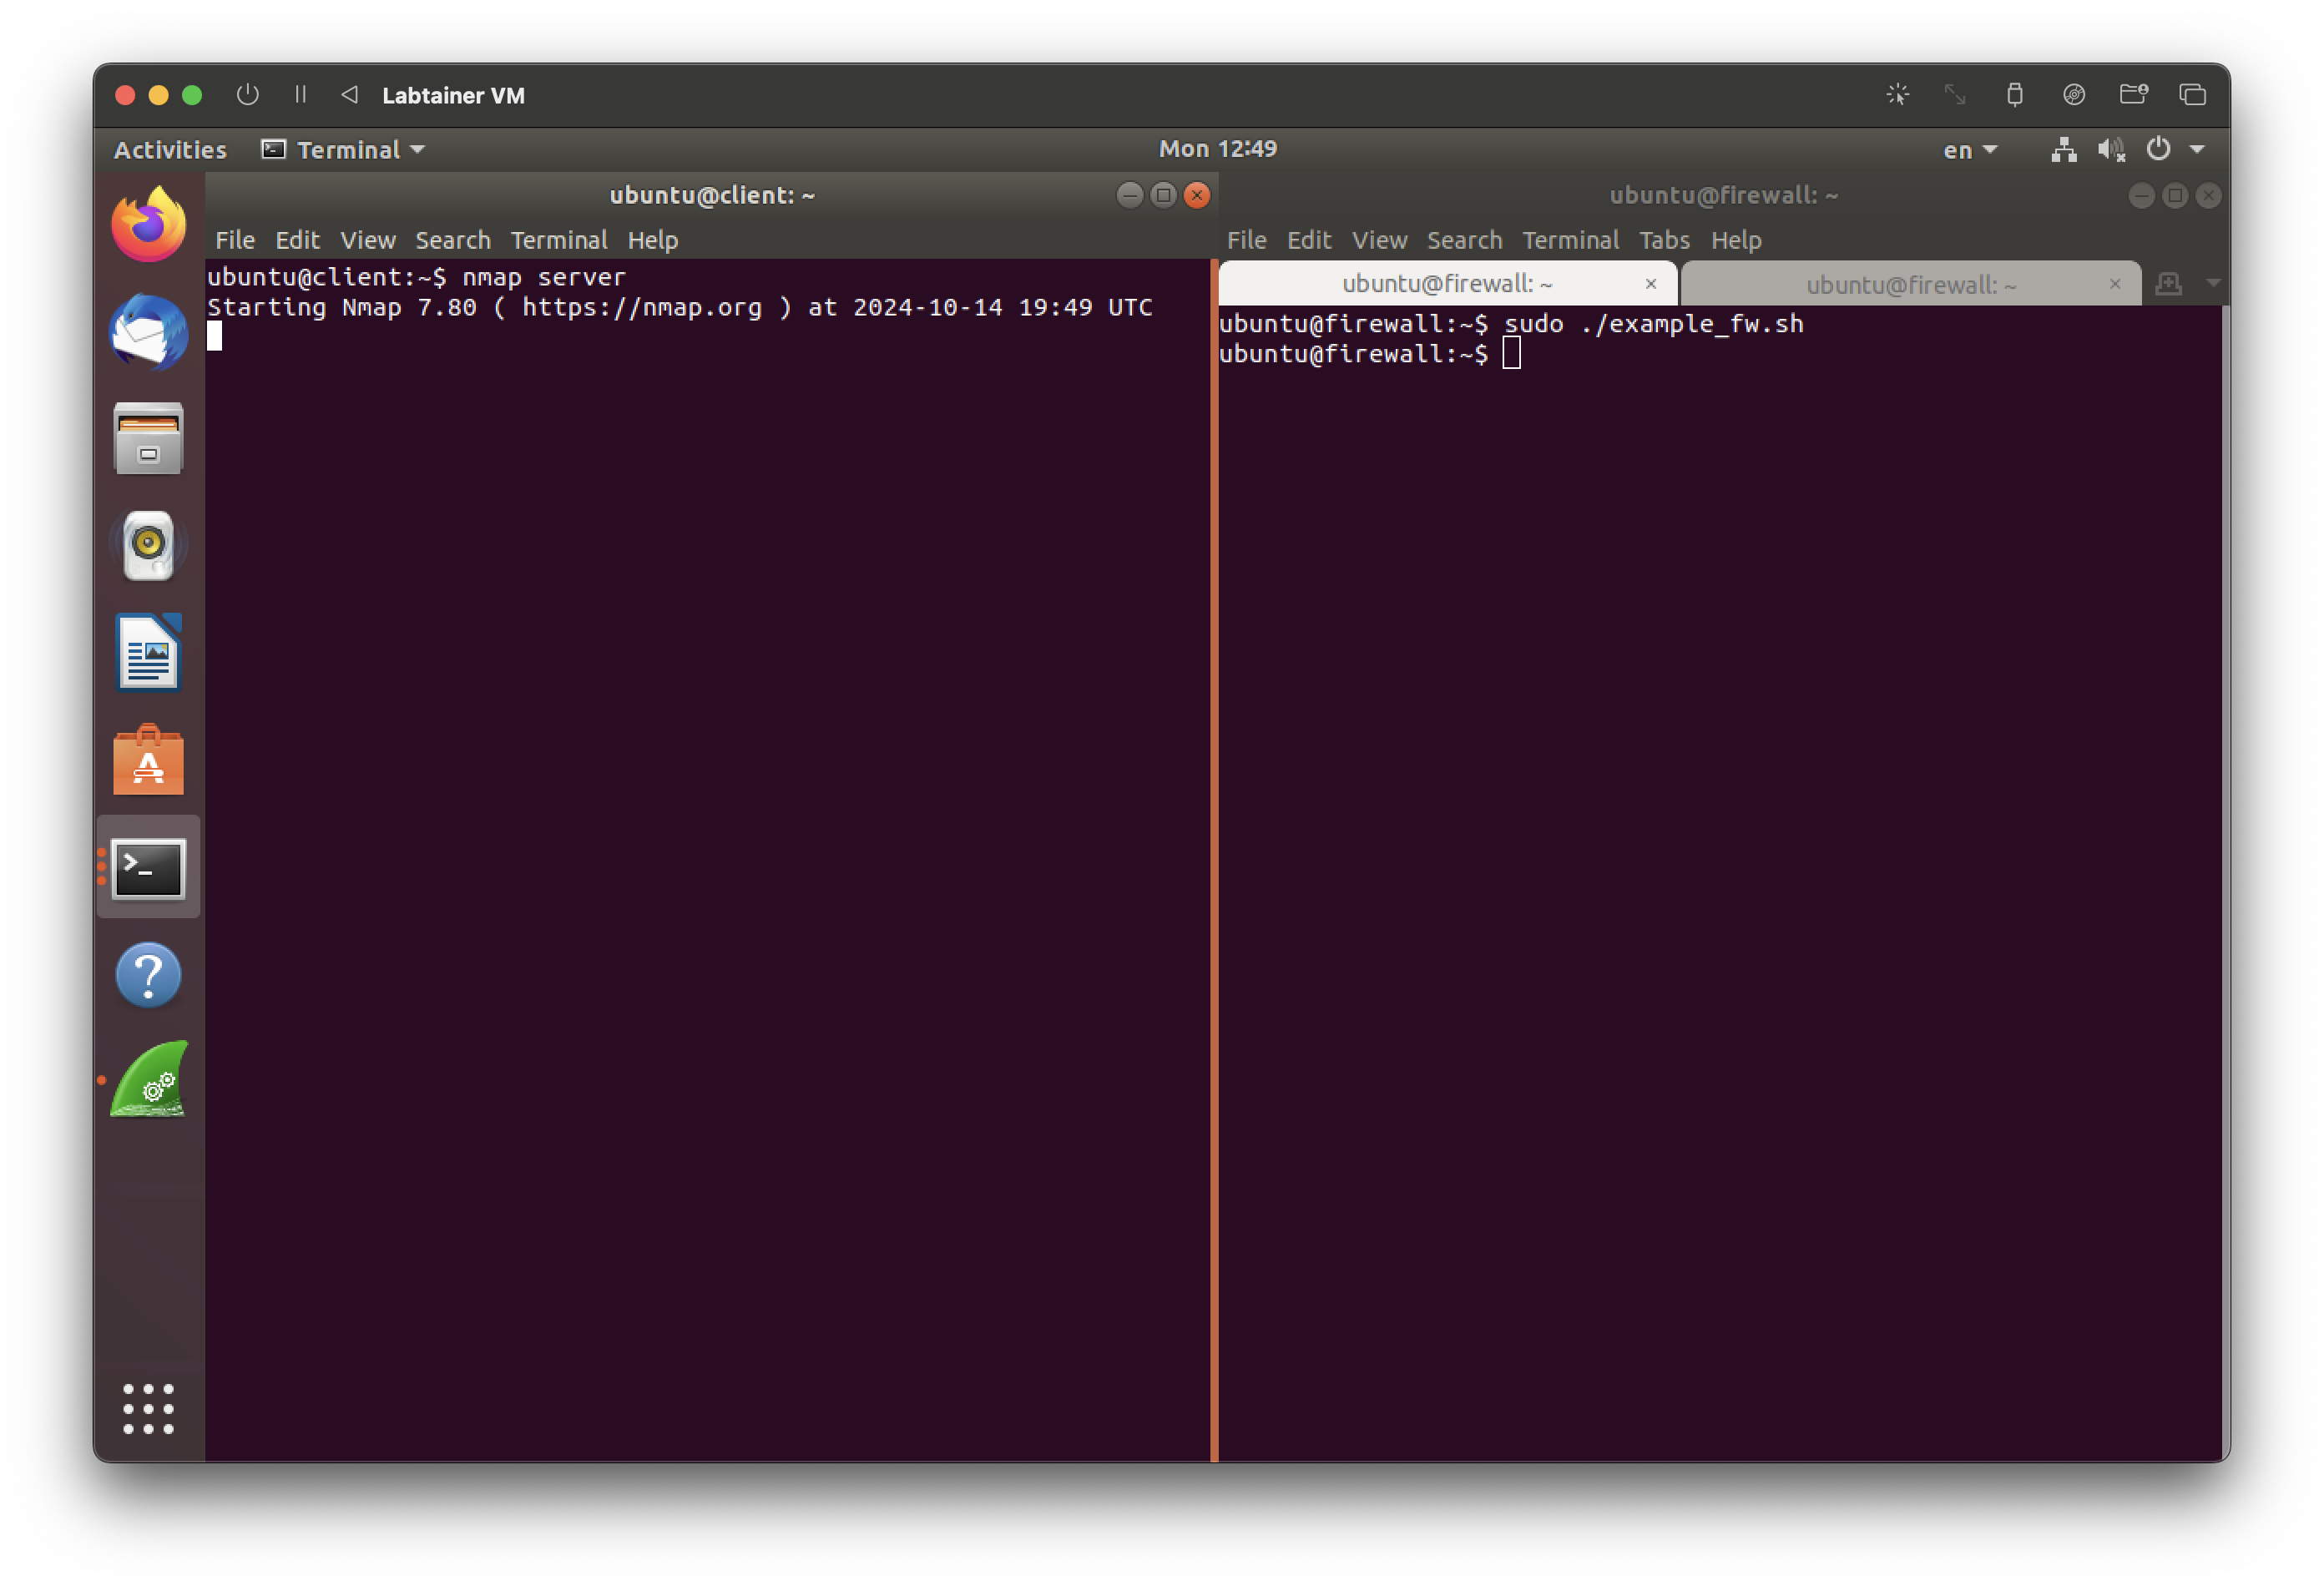
\includegraphics[width=0.8\textwidth]{/Users/marcalstorino/Documents/EMSE/MAJEUR 1 - INFORMATIQUE/Sécurité des Systèmes d'informations/Lab 02/JoaoPedroMarcalStorino_Lab02/image/img11.png} % Substitua pelo caminho correto da imagem
\caption{Verifying configuration with nmap}
\end{figure}

\subsection*{Step 4: Allow a New Service - wizbang}
In this step, we will modify the firewall to allow traffic on port 10015 for the \texttt{wizbang} service. On the firewall terminal, edit the IPTables configuration file with:

\begin{verbatim}
sudo nano wizbang
\end{verbatim}

Add the appropriate rules to allow traffic on port 10015, then save and exit the file. Verify the changes using:

\begin{verbatim}
nmap server
\end{verbatim}

% Imagem para wizbang tentando usar a porta 10015
\begin{figure}[h!]
\centering
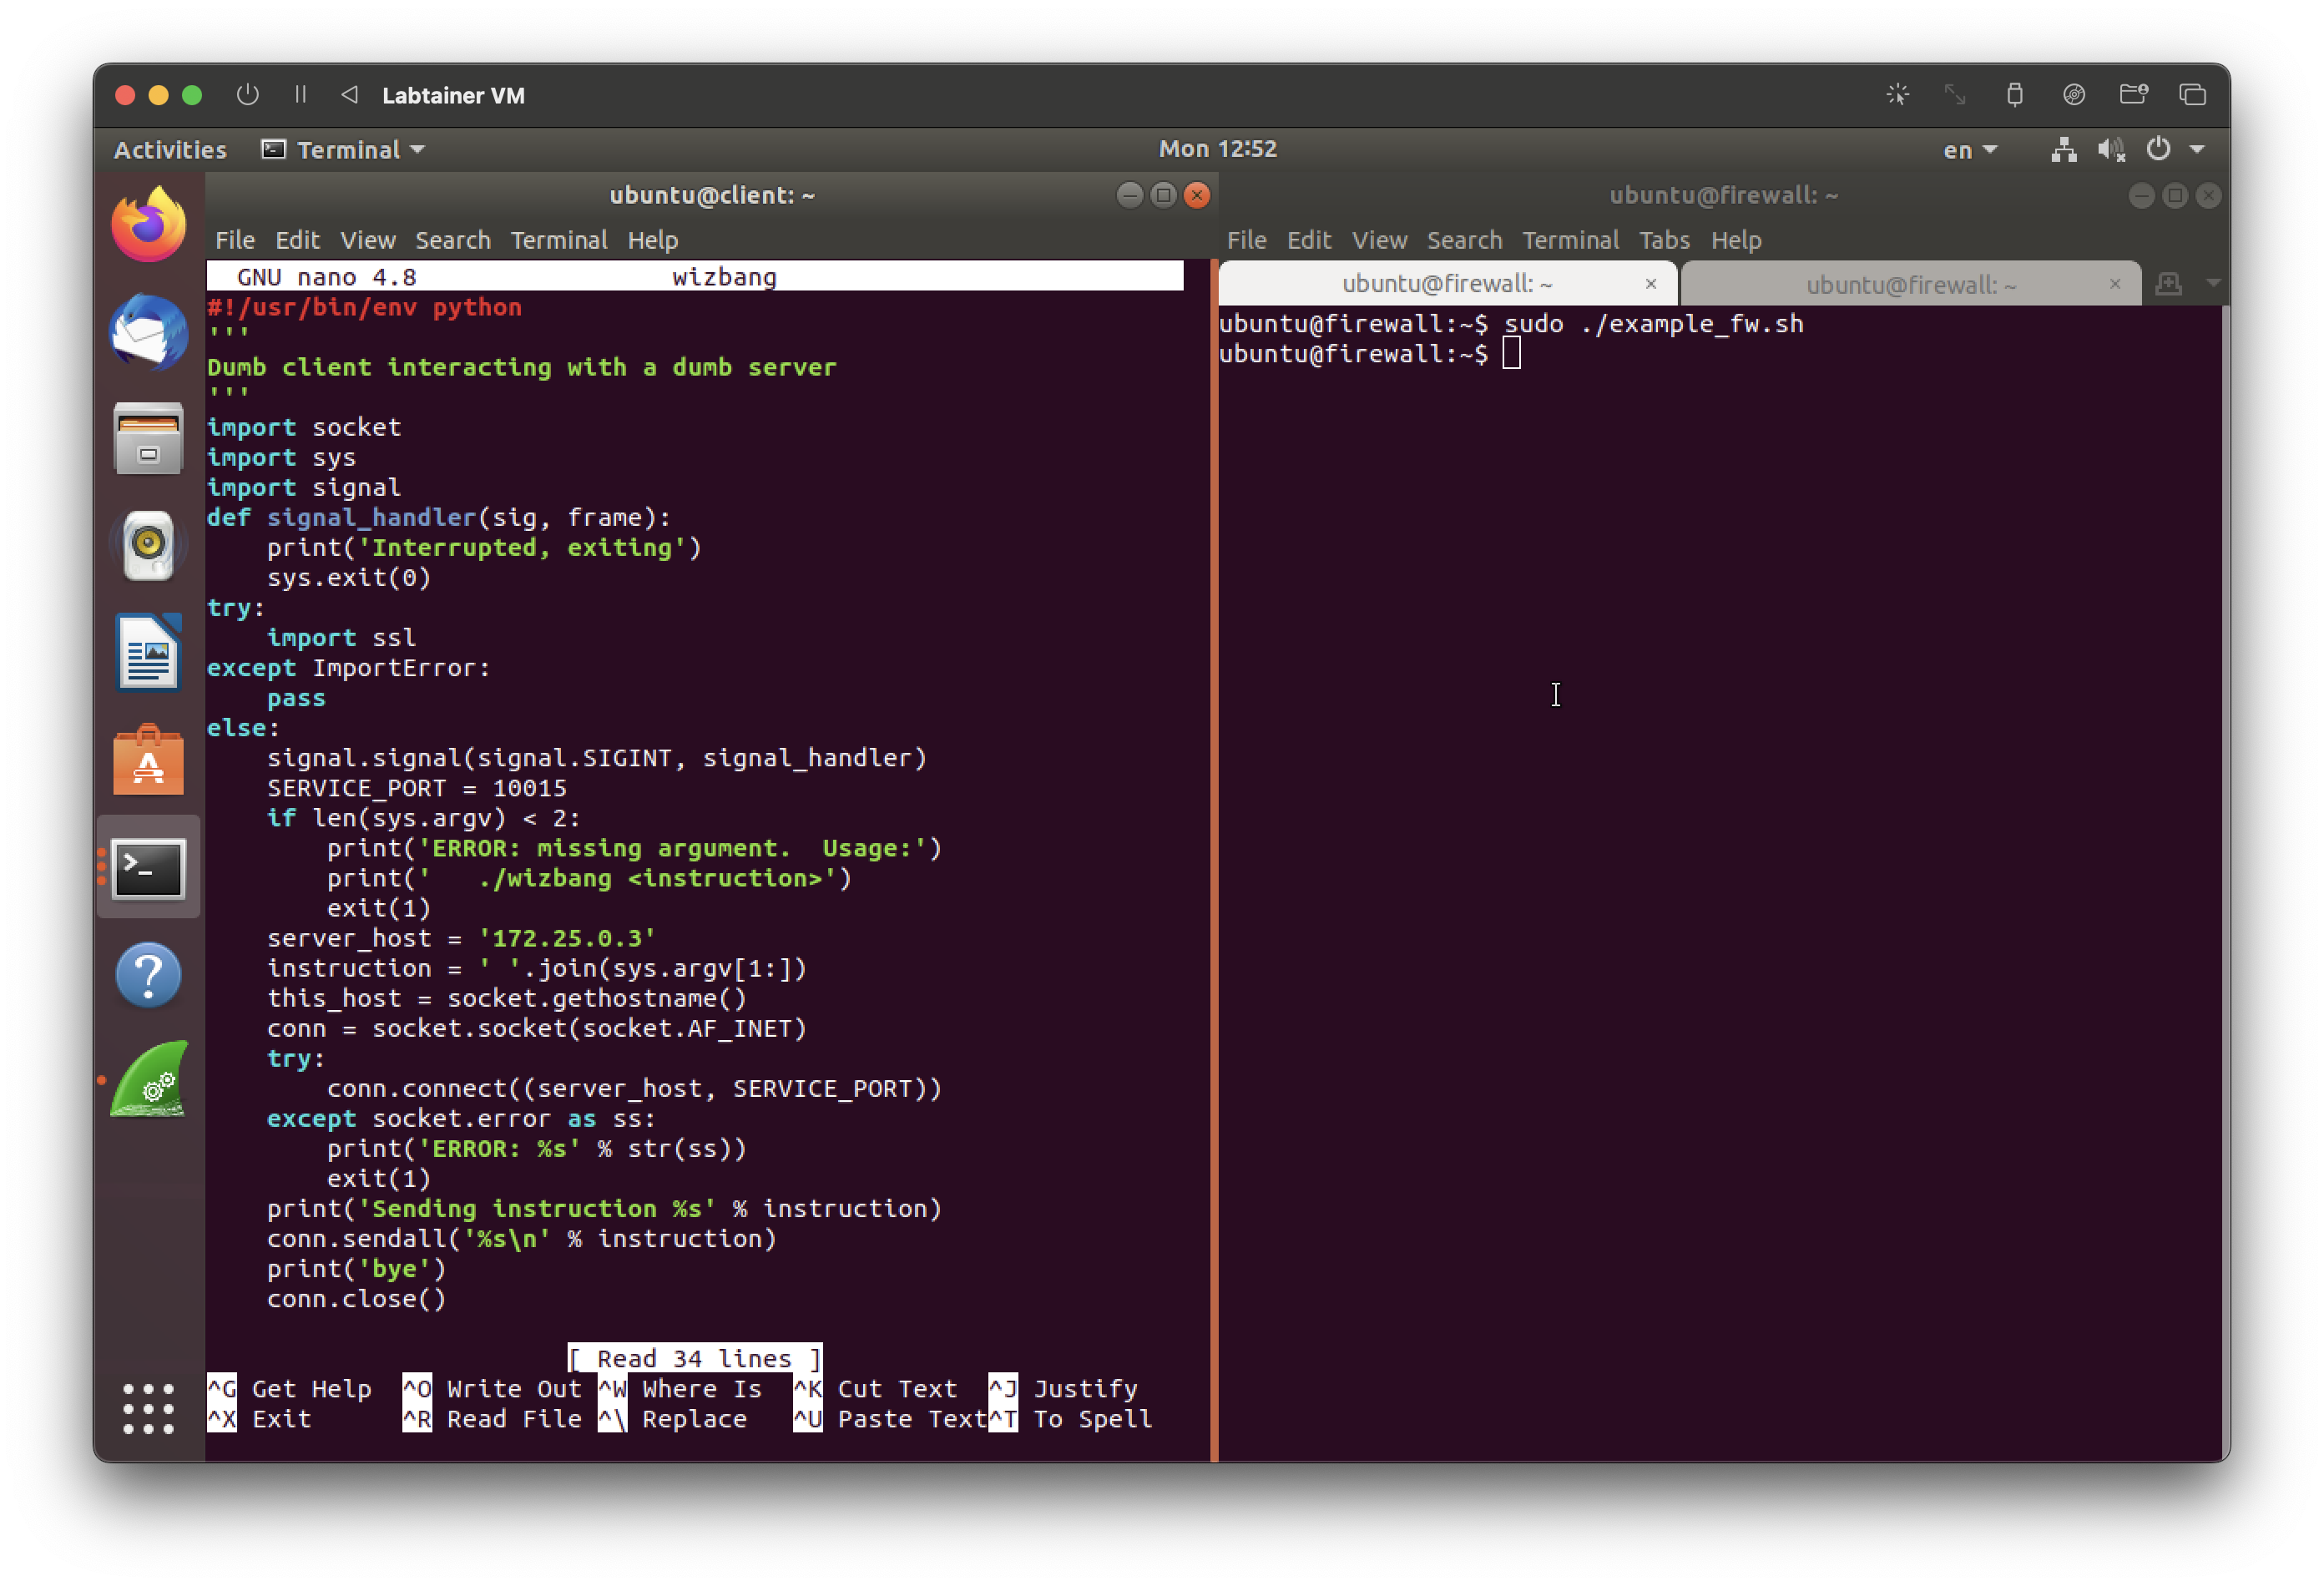
\includegraphics[width=0.8\textwidth]{/Users/marcalstorino/Documents/EMSE/MAJEUR 1 - INFORMATIQUE/Sécurité des Systèmes d'informations/Lab 02/JoaoPedroMarcalStorino_Lab02/image/img12.png} % Substitua pelo caminho correto da imagem
\caption{Attempting to use port 10015 with wizbang}
\end{figure}

% Imagem para alterar o documento para incluir a porta 10015
\begin{figure}[h!]
\centering
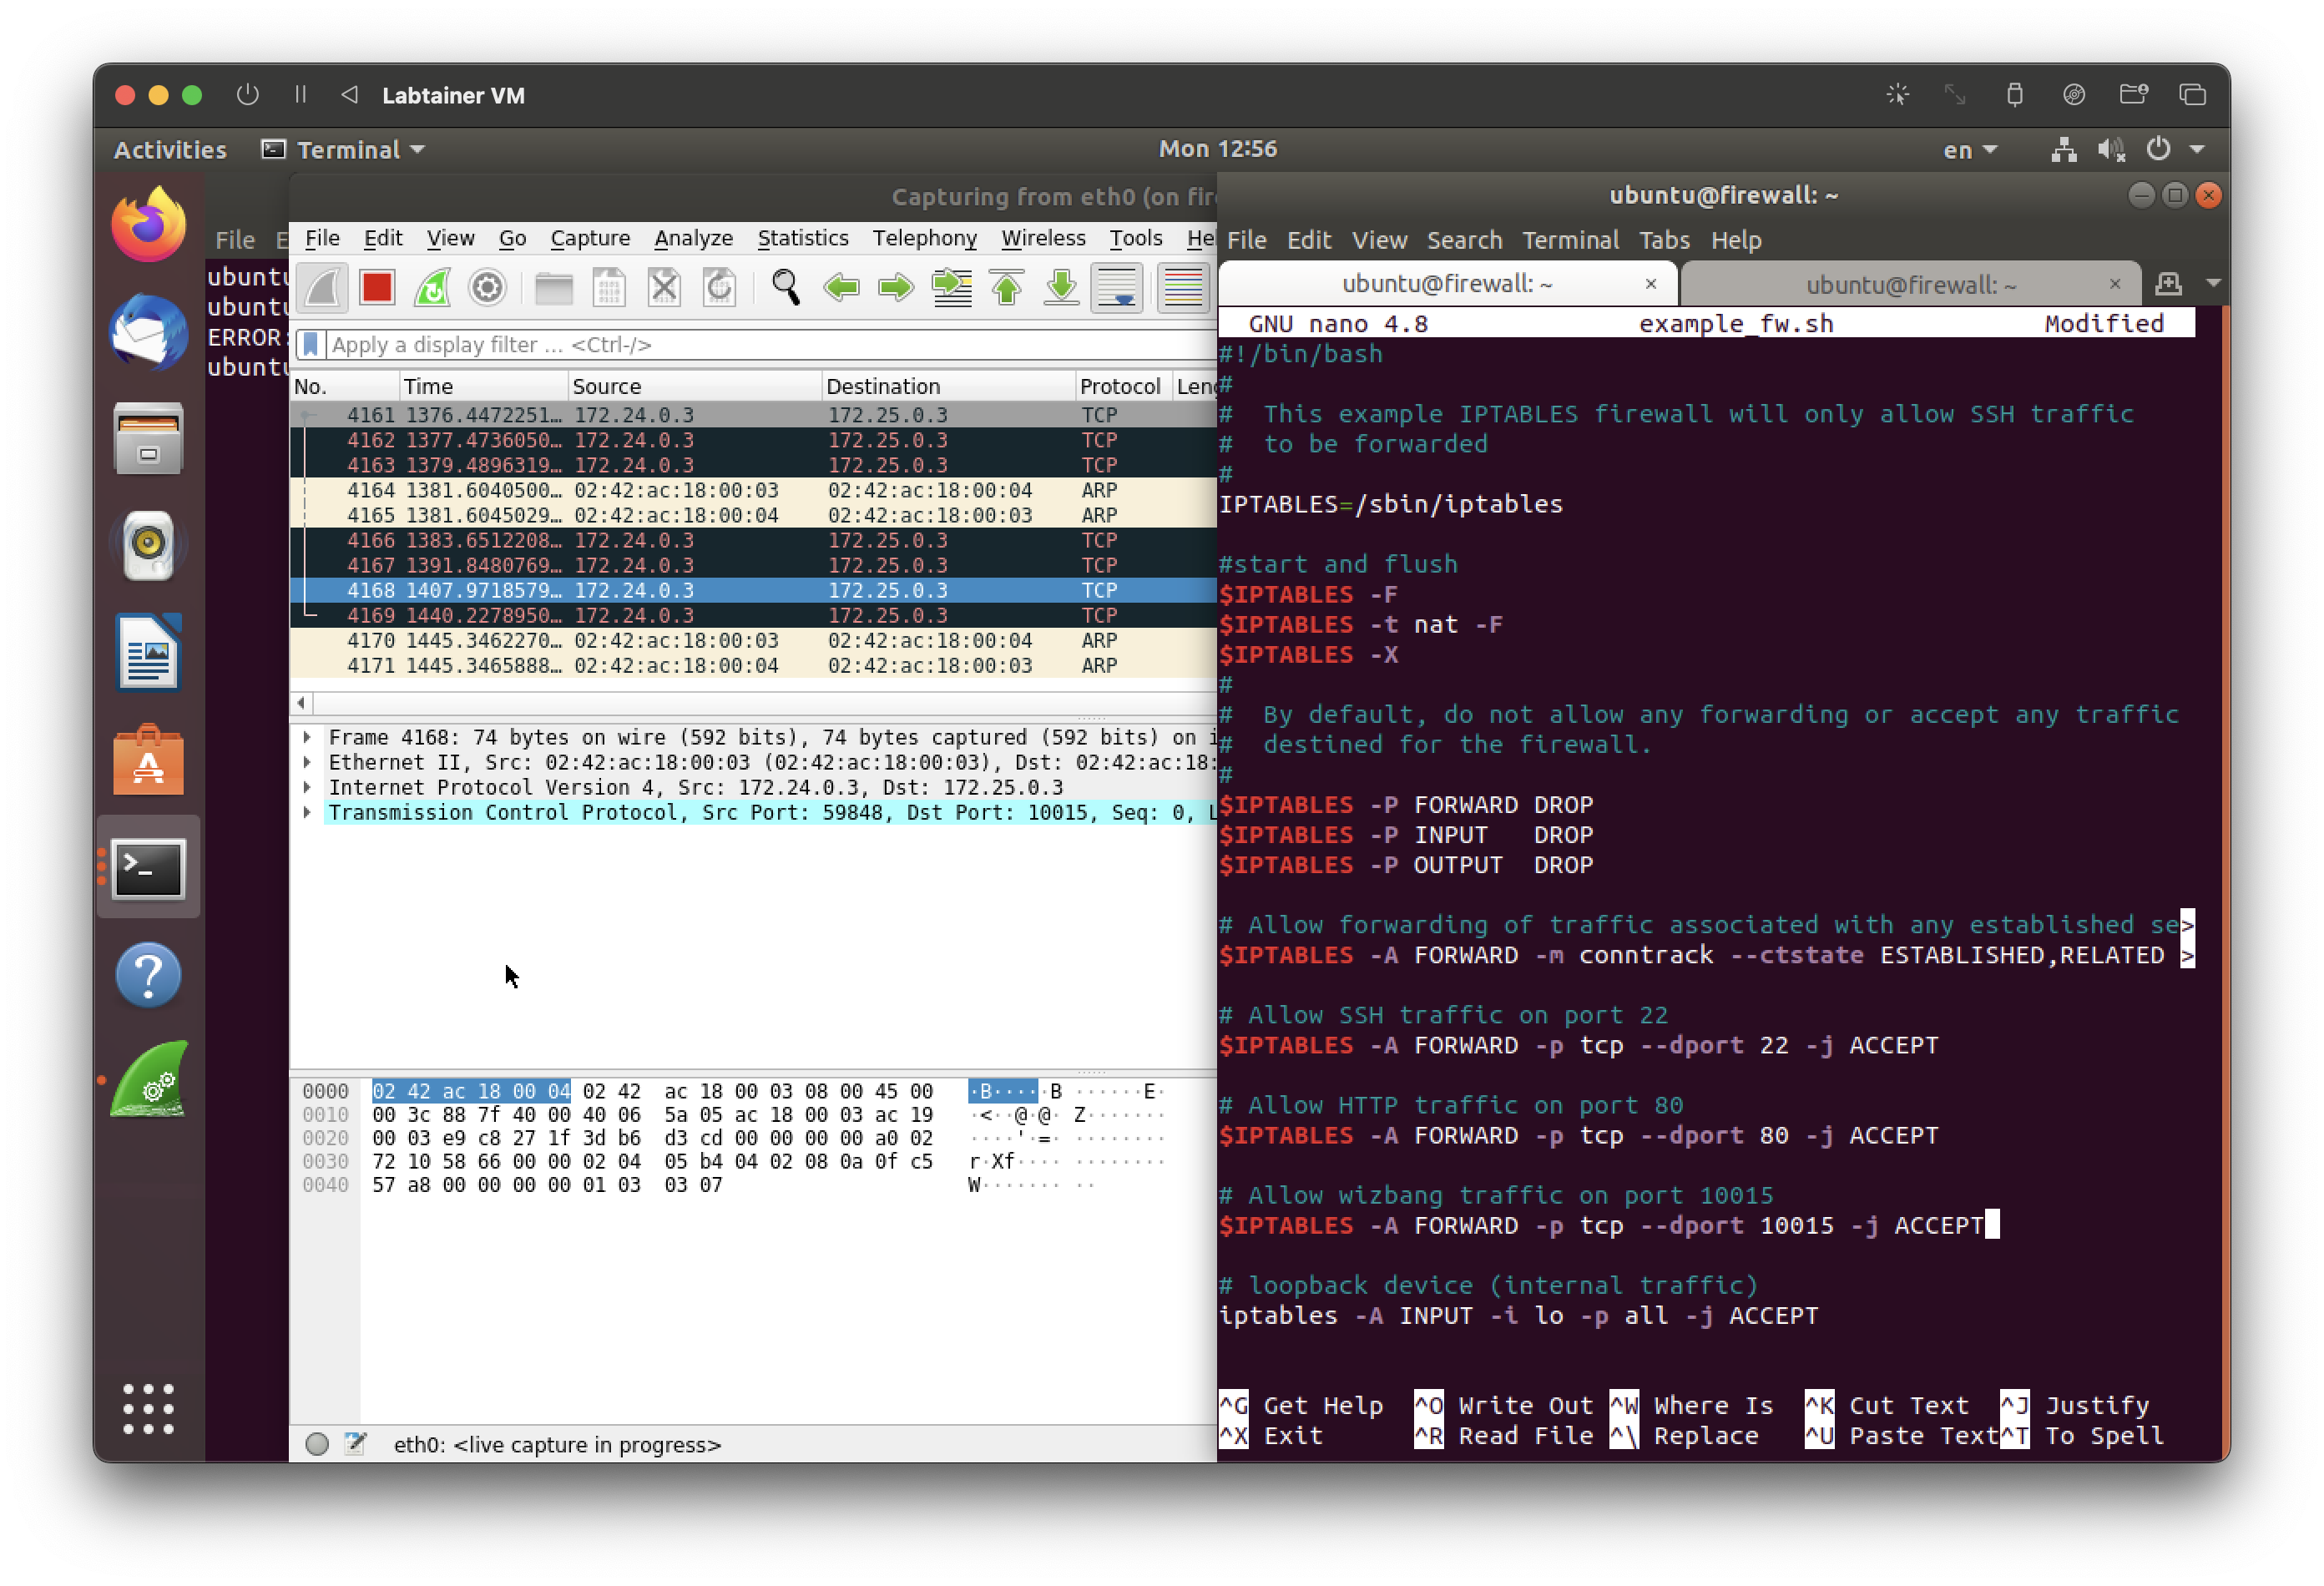
\includegraphics[width=0.8\textwidth]{/Users/marcalstorino/Documents/EMSE/MAJEUR 1 - INFORMATIQUE/Sécurité des Systèmes d'informations/Lab 02/JoaoPedroMarcalStorino_Lab02/image/img13.png} % Substitua pelo caminho correto da imagem
\caption{Modifying the IPTables configuration to include port 10015}
\end{figure}

% Imagem mostrando que deu certo
\begin{figure}[h!]
\centering
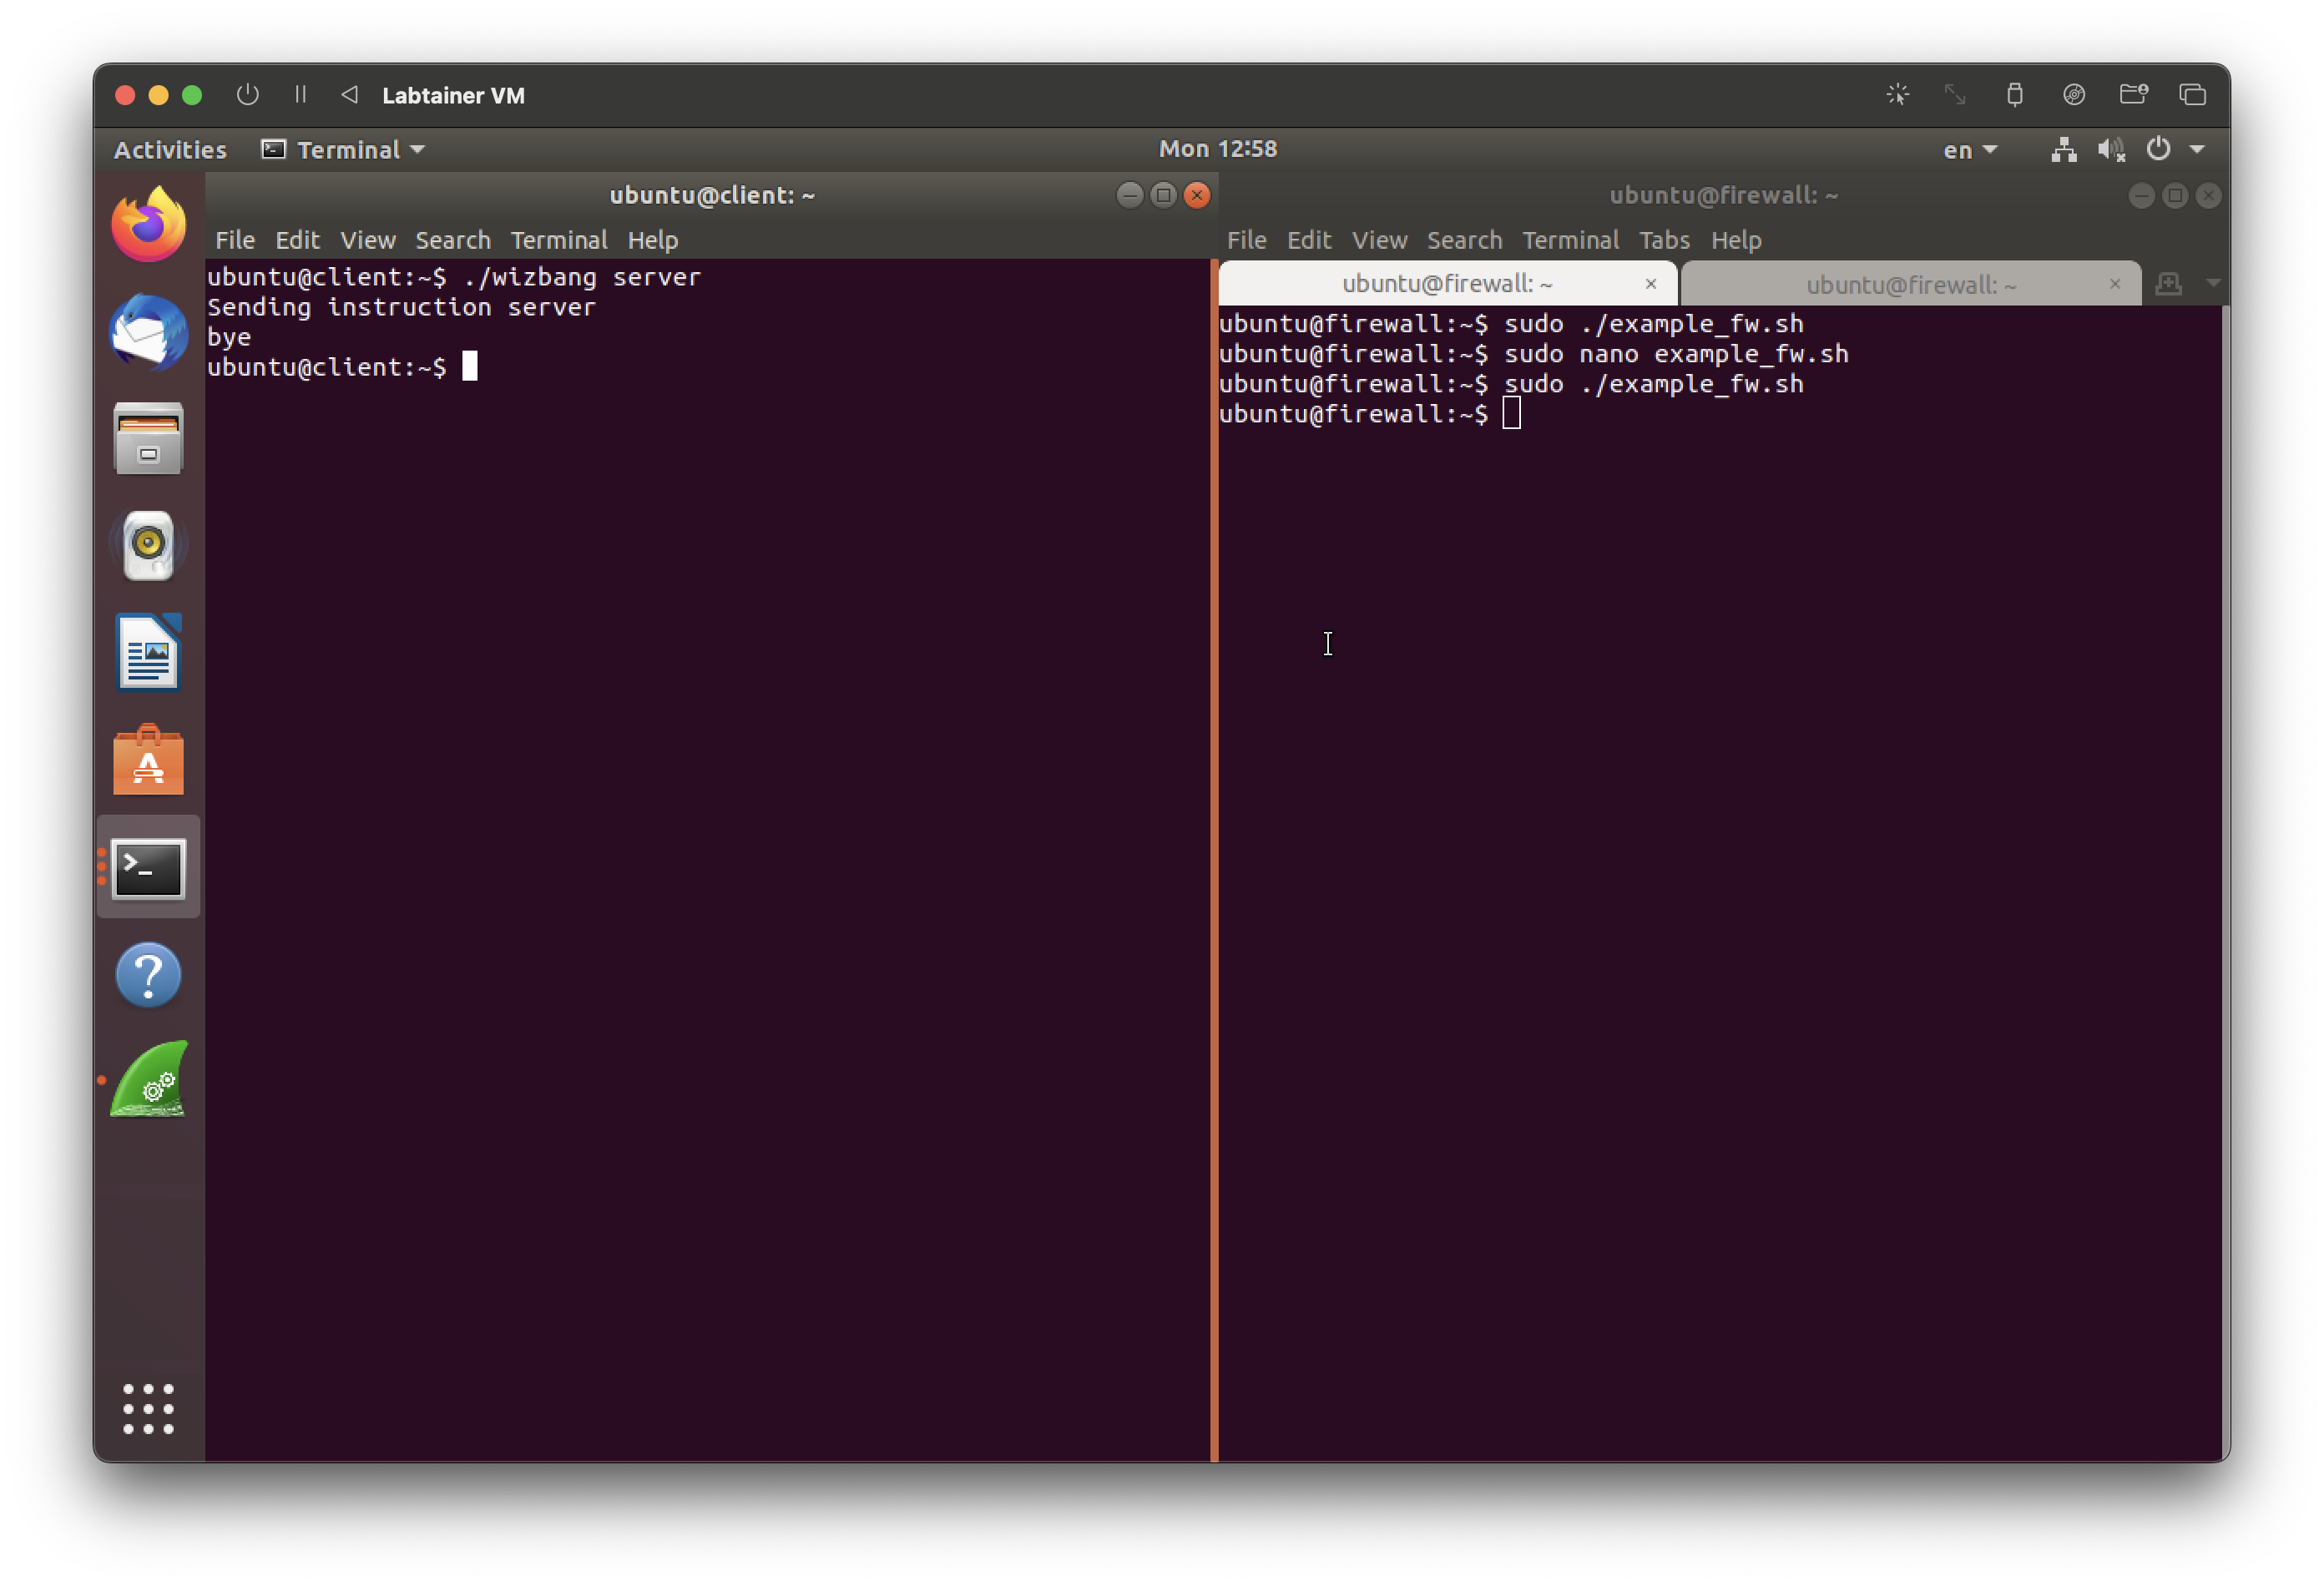
\includegraphics[width=0.8\textwidth]{/Users/marcalstorino/Documents/EMSE/MAJEUR 1 - INFORMATIQUE/Sécurité des Systèmes d'informations/Lab 02/JoaoPedroMarcalStorino_Lab02/image/img14.png} % Substitua pelo caminho correto da imagem
\caption{Successfully allowing traffic on port 10015 for wizbang}
\end{figure}

\subsection*{Step 5: Conclusion}
By completing this lab, we successfully configured a firewall using IPTables. We restricted traffic to only allow specific services, applied and tested firewall rules, and explored how to monitor network traffic using Wireshark. The ability to control traffic in a Linux environment is critical for securing networks and managing access.

\end{document}